\documentclass[aspectratio=169]{beamer}
% Shared preamble for ml/ slide decks.
% Each lecture .tex starts with:
%   \documentclass[aspectratio=169]{beamer}
%   \input{../preamble}
% Compile from inside the chapter folder so \input{../preamble} resolves.

\usetheme{default}
\usecolortheme{dove}

\setbeamertemplate{navigation symbols}{}
\setbeamertemplate{footline}{%
  \hfill{\large\insertframenumber\,/\,\inserttotalframenumber}\hspace{0.8em}\vspace{0.5em}%
}

% Project palette (existing, kept for backwards compatibility with deferred/*)
\definecolor{popblue}{RGB}{52, 101, 164}
\definecolor{sampred}{RGB}{204, 0, 0}
\definecolor{paramgreen}{RGB}{0, 140, 70}
\definecolor{warnred}{RGB}{180, 40, 40}
\definecolor{orange1}{RGB}{220, 120, 0}
\definecolor{violet1}{RGB}{120, 50, 160}
\definecolor{lightbg}{RGB}{245, 245, 250}

% Armenian flag palette (use these for any 3-color highlight; per CLAUDE.md).
% "Nice versions": slightly de-saturated from the official spec for slide use,
% so they don't burn out under projector colors. Originals kept as *_pure.
\definecolor{armred}{RGB}{200, 30, 40}      % nice red (official #D90012 muted)
\definecolor{armblue}{RGB}{30, 70, 160}     % nice blue (official #0033A0 muted)
\definecolor{armorange}{RGB}{230, 160, 30}  % nice orange (official #F2A800 muted)
\definecolor{armred_pure}{HTML}{D90012}     % official Armenian flag red
\definecolor{armblue_pure}{HTML}{0033A0}    % official Armenian flag blue
\definecolor{armorange_pure}{HTML}{F2A800}  % official Armenian flag orange

\setbeamercolor{frametitle}{fg=popblue}
\setbeamercolor{title}{fg=popblue}

\usepackage{pgfplots}
\usepackage{tikz}
\usetikzlibrary{shapes, arrows.meta, positioning, calc, decorations.pathreplacing, patterns, matrix}
\pgfplotsset{compat=1.18}
\usepackage{amsmath, amssymb, amsfonts}
\usepackage{bm}
\usepackage{dsfont}
\usepackage{array}
\usepackage{pifont}
\usepackage{colortbl}
\usepackage{fontenc}

% Callout boxes. Purely additive - existing decks are unaffected.
% Usage: \begin{tcolorbox}[colback=armblue!8, colframe=armblue, boxrule=0.6pt, arc=2pt,
%                          title=\textbf{Key idea}] ... \end{tcolorbox}
% Palette convention (ml/SLIDE_STYLE.md): armblue=key idea, armred=trap/warning,
% paramgreen=takeaway or "Next", armorange=watch-out.
\usepackage[most]{tcolorbox}

% Cleaner table rules (\toprule, \midrule, \bottomrule). Also purely additive.
\usepackage{booktabs}

% \cancel{...} for struck-through terms in derivations (added 2026-08-11 for the
% importance-sampling frame in ch11_rl, where the dynamics cancel). Purely additive.
\usepackage{cancel}

% Minimal ML notation macros (subset of slds-lmu latex-math/basic-ml.tex).
% Kept here so we don't have to inline-expand every \thetav, \xv, etc.
% when porting upstream slides.
\newcommand{\R}{\mathds{R}}
\newcommand{\N}{\mathds{N}}
\newcommand{\E}{\mathds{E}}
\newcommand{\Xspace}{\mathcal{X}}
\newcommand{\Yspace}{\mathcal{Y}}
\newcommand{\Hspace}{\mathcal{H}}
\newcommand{\D}{\mathcal{D}}
\newcommand{\Dtrain}{\mathcal{D}_{\text{train}}}
\newcommand{\Dtest}{\mathcal{D}_{\text{test}}}
\newcommand{\xv}{\mathbf{x}}
\newcommand{\yv}{\mathbf{y}}
\newcommand{\Xmat}{\mathbf{X}}
\newcommand{\id}{\mathbf{I}}
\newcommand{\thetav}{\bm{\theta}}
\newcommand{\thetah}{\hat{\bm{\theta}}}
\newcommand{\lamv}{\bm{\lambda}}
\newcommand{\fx}{f(\xv)}
\newcommand{\fxt}{f(\xv \,|\, \bm{\theta})}
\newcommand{\fxi}{f\!\left(\xv^{(i)}\right)}
\newcommand{\fh}{\hat{f}}
\newcommand{\fxh}{\hat{f}(\xv)}
\newcommand{\yh}{\hat{y}}
\newcommand{\yih}{\hat{y}^{(i)}}
% \xi clashes with the Greek letter \xi; write \xv^{(i)} inline instead.
\newcommand{\yi}[1][i]{y^{(#1)}}
\newcommand{\xyi}[1][i]{\left(\xv^{(#1)},\, y^{(#1)}\right)}
\newcommand{\thx}{\bm{\theta}^\top \xv}
\newcommand{\sumin}{\sum_{i=1}^{n}}
\newcommand{\sumjp}{\sum_{j=1}^{p}}
\newcommand{\Lxy}{L\!\left(y, \fx\right)}
\newcommand{\Lxyi}{L\!\left(\yi, \fxi\right)}
\newcommand{\risk}{\mathcal{R}}
\newcommand{\riske}{\mathcal{R}_{\text{emp}}}
\newcommand{\risket}{\mathcal{R}_{\text{emp}}(\bm{\theta})}
\newcommand{\riskt}{\mathcal{R}(\bm{\theta})}
\newcommand{\riskr}{\mathcal{R}_{\text{reg}}}
\newcommand{\argmin}{\mathop{\mathrm{arg\,min}}}
\newcommand{\argmax}{\mathop{\mathrm{arg\,max}}}
\newcommand{\eps}{\varepsilon}


\graphicspath{{fig/}{../00_shared/fig/}}

% callout boxes, matching LLM-1 and LLM-3/LLM-4's fcolorbox house pattern
\newcommand{\keybox}[1]{\fcolorbox{armblue}{armblue!8}{\parbox{0.97\linewidth}{\small #1}}}
\newcommand{\trapbox}[1]{\fcolorbox{armred}{armred!8}{\parbox{0.97\linewidth}{\small #1}}}
\newcommand{\takebox}[1]{\fcolorbox{paramgreen}{paramgreen!8}{\parbox{0.97\linewidth}{\small #1}}}
\newcommand{\watchbox}[1]{\fcolorbox{armorange}{armorange!12}{\parbox{0.97\linewidth}{\small #1}}}

\newcommand{\sectiontransition}[2]{%
  \begin{frame}[plain]
    \vfill
    \begin{center}
      {\Huge\bfseries\color{popblue} #1}\\[1.1em]
      {\large #2}
    \end{center}
    \vfill
  \end{frame}}

\newcommand{\src}[1]{{\scriptsize\color{gray} #1}}
% one panel cropped out of emb_gpt2_positions.pdf, with one rectangle whited out (corners as
% fractions of the cropped image): the neighbouring panel's label overlaps the crop
\newcommand{\gptpanel}[6]{%
  \begin{tikzpicture}
    \node[anchor=south west, inner sep=0] (im)
      {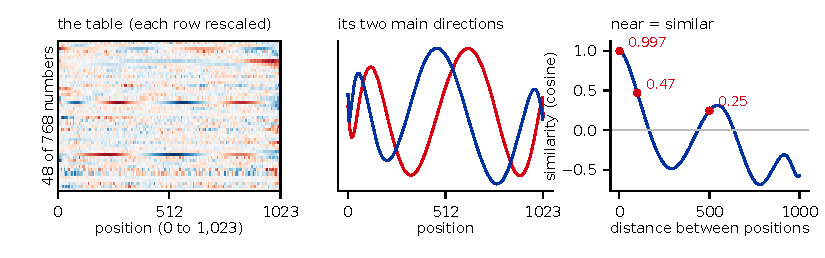
\includegraphics[width=#1,trim=#2,clip]{emb_gpt2_positions.pdf}};
    \begin{scope}[x={(im.south east)}, y={(im.north west)}]
      \fill[white] (#3,#4) rectangle (#5,#6);
    \end{scope}
  \end{tikzpicture}}
\newcommand{\link}[2]{\href{#1}{\textcolor{popblue}{#2}}}   % no underline: long titles must break

\title{Embeddings and position}
\subtitle{From IDs to vectors}
\author{}
\date{}

\begin{document}

\begin{frame}[plain]
  \titlepage
  \begin{center}\scriptsize\color{gray}
    LLM chapter, session 2. Every GPT-2 (2019) number on these slides is read from its real weights.
  \end{center}
\end{frame}

% ============================================================ LINKS (2026-10-27, as in LLM-1)
\begin{frame}{Before we start: two videos and a demo}
  \begin{columns}[T]
    \column{0.49\textwidth}
    \keybox{\raggedright\textbf{Recommended viewing}\\[4pt]
    3Blue1Brown,
    \link{https://youtu.be/wjZofJX0v4M?t=747}{Transformers, the tech behind LLMs \textbar{} Deep
    Learning Chapter 5} (2024). From 12:27: word embeddings as directions in space.\\[6pt]
    Jia-Bin Huang,
    \link{https://www.youtube.com/watch?v=SMBkImDWOyQ}{How Rotary Position Embedding Supercharges
    Modern LLMs [RoPE]} (2024, 14 min). Sinusoids, then RoPE, then stretching it: today's second
    half, in the same order.}
    \column{0.49\textwidth}
    \takebox{\raggedright\textbf{Live demo:}
    \link{https://projector.tensorflow.org}{projector.tensorflow.org}\\[4pt]
    10,000 word vectors (word2vec, 2013; 200 numbers each) in the browser: search a word, list its
    nearest neighbours, squash all 10,000 into 3-D with PCA (ch10), t-SNE (2008) or UMAP (2018).}
    \vskip 4pt
    {\small\textbf{Try:}}
    \begin{itemize}\small
      \item a weekday, a city, a royal title
      \item an adjective: is its opposite among the neighbours?
      \item switch PCA to UMAP and watch clusters form
    \end{itemize}
  \end{columns}
\end{frame}

% ============================================================ WHERE WE ARE (py_src/llm_roadmap.py)
\begin{frame}{Where we are: one forward pass}
  \begin{center}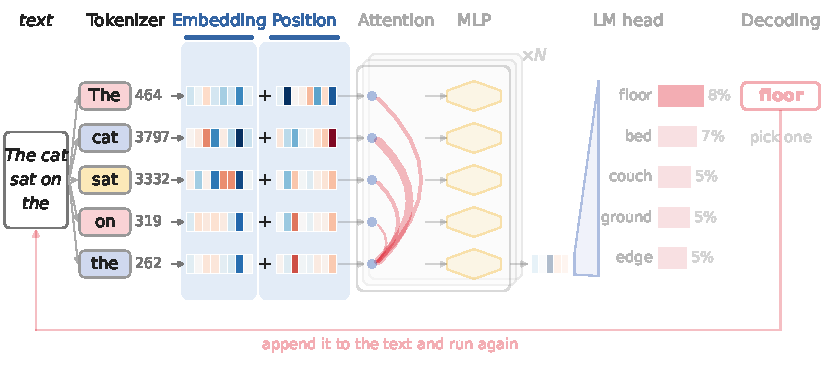
\includegraphics[width=\linewidth]{roadmap_embeddings_pass.pdf}\end{center}
  \vskip -2pt
  {\small Today: the next two boxes - an ID becomes a vector, and the vector learns where it sits.}
\end{frame}

\begin{frame}{Where we are: the life of a model}
  \begin{center}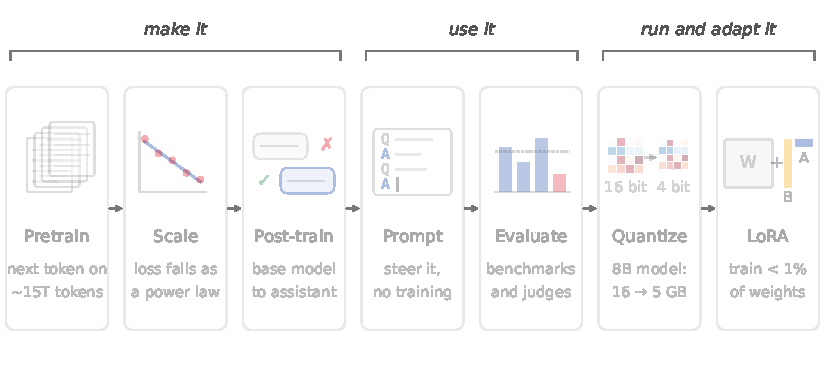
\includegraphics[width=\linewidth]{roadmap_embeddings_life.pdf}\end{center}
  \vskip -2pt
  {\small Later: where the weights come from, and what you do with them once you have them.}
\end{frame}

% ============================================================ COLD OPEN
\begin{frame}{Same words, opposite news}
  \begin{center}
    {\Large ``The dog bites the man''}\\[4pt]
    {\Large ``The man bites the dog''}
  \end{center}
  \vskip 2pt
  \textbf{Predict:} the model's first step looks every token up in a table and gets back a list of
  numbers. Are the two sentences still different after that step?
  \vfill
  \begin{center}
    
\includegraphics[width=3.0in]{emb_kargin.pdf}\\[-2pt]
    \src{\href{https://karginhaghordum.am/sketch/3bEwVKXicsQ/}{karginhaghordum.am/sketch/3bEwVKXicsQ}}
  \end{center}
\end{frame}

\begin{frame}{Same five numbers, same five vectors}
  \begin{center}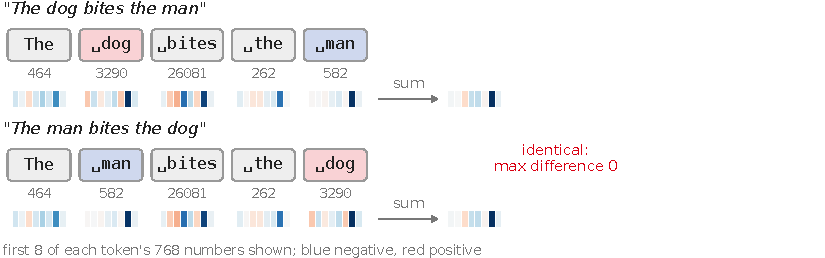
\includegraphics[width=\linewidth]{emb_coldopen_ids.pdf}\end{center}
  \vskip -4pt
  {\small The same five token IDs in a different order. Each ID fetches its row of the table, so
  both sentences arrive as the \textbf{same five vectors}. Add them up and the totals agree to
  the last bit.}
  \vskip 4pt
  \watchbox{Aside: without ``The'', ``dog bites man'' and ``man bites dog'' are not even the same
  tokens. The first word has no space before it, and ``dog'' is a different token from ``\,dog''
  (LLM-1).}
\end{frame}

\begin{frame}{Outline}
  \tableofcontents
\end{frame}

% ============================================================ 1. ID -> VECTOR
\section{An ID becomes a vector}
\sectiontransition{An ID becomes a vector}{3290 is a row number, not a quantity.}

\begin{frame}{An ID is a name, not a number}
  \begin{itemize}
    \item LLM-1 ended with integers: `` cat'' is \textbf{3797}, `` dog'' is \textbf{3290}.
    \item Is a cat 507 ``more'' than a dog? Is `` dog'' + 1 a puppy? The IDs were handed out by
      the order of BPE's merges (Sennrich et al., 2016; LLM-1). Their sizes mean nothing.
    \item{} [53] hit the same wall with one-hot vectors: every word equally far from every other,
      so ``cat'' is no closer to ``dog'' than to ``Tuesday''.
  \end{itemize}
  \vskip 10pt
  \keybox{What we want: one list of numbers per token, where tokens used in similar ways get
  similar numbers. And we want the model to \textbf{learn} those numbers, not us to choose them.}
\end{frame}

\begin{frame}{By hand: a one-hot vector times a matrix picks a row}
  \small
  A 4-token vocabulary (the, cat, sat, on), 3 numbers per token. The table $E$ has one row per
  token. ``cat'' is token 1, so its one-hot vector has a 1 in place 1:
  \[
    \underbrace{\begin{pmatrix} 0 & 1 & 0 & 0 \end{pmatrix}}_{\text{one-hot(cat)}}
    \underbrace{\begin{pmatrix}
      \phantom{-}0.2 & -0.1 & \phantom{-}0.5 \\
      \phantom{-}0.9 & \phantom{-}0.3 & -0.4 \\
      -0.6 & \phantom{-}0.8 & \phantom{-}0.1 \\
      \phantom{-}0.0 & -0.5 & \phantom{-}0.7
    \end{pmatrix}}_{E \text{ (4 tokens} \times \text{3 numbers)}}
    = 0 \cdot \text{row}_0 + 1 \cdot \text{row}_1 + 0 \cdot \text{row}_2 + 0 \cdot \text{row}_3
    = \begin{pmatrix} 0.9 & 0.3 & -0.4 \end{pmatrix}
  \]
  \vskip -2pt
  \begin{itemize}
    \item Every zero wipes out a row; the single 1 keeps row 1. So the ``embedding layer'' is a
      matrix multiplication that is really a \textbf{table lookup}: code just reads row 1.
    \item Training works the same way: the gradient reaches only the rows that were looked up.
      A token that never shows up in training never moves.
  \end{itemize}
\end{frame}

\begin{frame}{GPT-2's table}
  \begin{columns}[T]
    \begin{column}{0.40\textwidth}
      \small
      \begin{itemize}
        \item One row per token: \textbf{50,257} rows.
        \item 768 numbers per row.
        \item $50{,}257 \times 768 = 38{,}597{,}376$ numbers: \textbf{31.0\%} of GPT-2 small's
          124M parameters (LLM-1's vocabulary trade-off).
      \end{itemize}
    \end{column}
    \begin{column}{0.58\textwidth}
      \vskip -2pt
      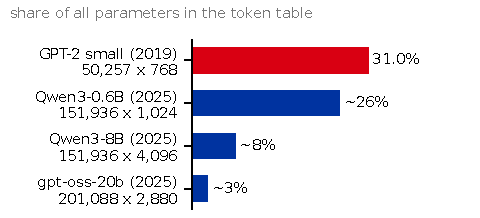
\includegraphics[width=\linewidth]{emb_table_sizes.pdf}
    \end{column}
  \end{columns}
  \vskip 8pt
  {\small Bigger models spend a smaller share on it: the table grows with the vocabulary and the
  width, the rest of the model grows much faster.}
  \vskip 2pt
  \src{Qwen3 and gpt-oss: vocabulary and width from their config.json, totals from their model
  cards (rounded there, hence ``\textasciitilde''), checked 4 Oct 2026.}
\end{frame}

\begin{frame}{Who fills the table?}
  \begin{itemize}
    \item At the start: small random numbers. ``cat'' and ``dog'' are as unrelated as any two
      rows.
    \item Then the table trains with the rest of the model, by backpropagation, on one task:
      predict the next token. Nobody ever tells it what a cat is.
    \item You have built one already: the ch11 name inventor was \textbf{an embedding table plus
      an MLP}. Its table had 40 rows (38 letters, plus the start and end symbols). Same idea,
      now with 50,257 rows.
  \end{itemize}
  \vskip 10pt
  \keybox{If two tokens keep appearing in the same places, the gradient keeps pushing their
  rows in the same direction. Similar use $\Rightarrow$ similar rows. Let us check whether that
  happened.}
\end{frame}

\begin{frame}{Predict first}
  \vskip 30pt
  \begin{center}
    {\Large\color{popblue}\textbf{Which rows of GPT-2's table sit closest to `` Monday''?}}
    \vskip 14pt
    {\small Closest = largest cosine similarity (the angle between two rows).}
    \vskip 24pt
    {\small\color{gray}Commit to an answer.}
  \end{center}
\end{frame}

\begin{frame}{What the table learned}
  \begin{center}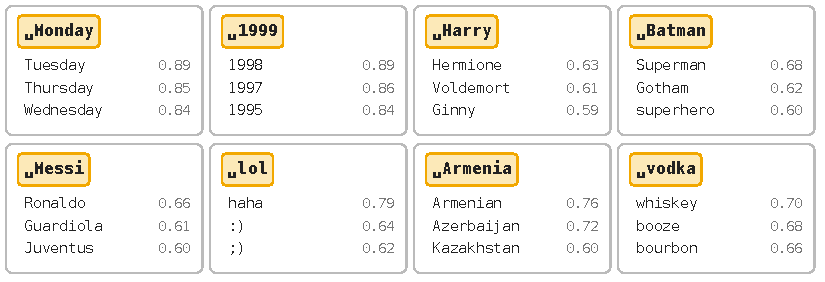
\includegraphics[width=\linewidth]{emb_neighbours.pdf}\end{center}
  \vskip -4pt
  {\small The three nearest rows of each word, with their cosine similarity. Days next to days,
  years next to years, Hermione next to Harry, Ronaldo next to Messi. Spelling variants of the
  word itself are skipped here (next slide).}
  \vskip 4pt
  \takebox{Nobody labelled a single token. All of this came from predicting the next one.}
\end{frame}

\begin{frame}{Neighbours share contexts, not meanings}
  \begin{center}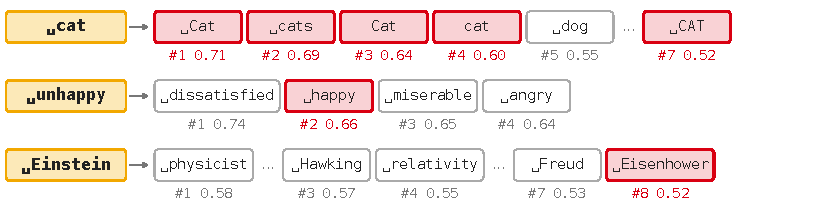
\includegraphics[width=0.88\linewidth]{emb_neighbours_odd.pdf}\end{center}
  \vskip -4pt
  \small
  \begin{itemize}
    \item `` cat'': the nearest rows are the same word spelled differently. LLM-1's tokenizer
      gave them separate IDs; training pulled their rows back together.
    \item `` unhappy'': its second neighbour is its \textbf{opposite}. ``I was \underline{\ \ \ \ }
      with the result'' takes both. Opposites live in the same places.
    \item `` Einstein'': physicists, then at \#8 `` Eisenhower'': another famous 20th-century
      name, with similar letters. Not physics.
  \end{itemize}
  \vskip 2pt
  \watchbox{A row records how a token is \textbf{used}. Usually that tracks meaning. Not always.
  Linguists said it in 1957: ``You shall know a word by the company it keeps'' (Firth).}
\end{frame}

\begin{frame}{The glitch tokens found each other}
  \begin{center}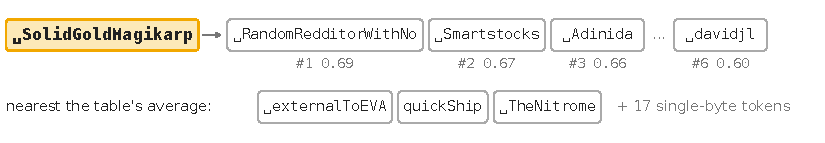
\includegraphics[width=\linewidth]{emb_glitch.pdf}\end{center}
  \vskip -2pt
  \small
  \begin{itemize}
    \item LLM-1's glitch token's nearest rows are \textbf{other glitch tokens}: Reddit user names
      and scraped-page leftovers.
    \item The 20 rows closest to the table's average row: these three, plus 17 single-byte
      tokens.
    \item Why: these tokens were in the tokenizer's training text and almost never in the
      model's. Their rows got no gradient of their own (the lookup slide), only the push every
      absent token gets at the output, where the same table scores the next token (tying, a few
      slides on): ``not this one''. That push points the same way for all of them, so they drifted
      together, toward the table's average.
  \end{itemize}
  \vskip 2pt
  \src{Land \& Bartolo (2024), ``Fishing for Magikarp'', EMNLP: thousands of such under-trained
  tokens in today's open models, found from the weights alone.}
\end{frame}

\begin{frame}{Directions carry meaning (mostly)}
  \small
  Take row $b$, subtract row $a$, add row $c$, and ask which row is nearest:
  \vskip 4pt
  \begin{center}
  \begin{tabular}{lll}
    \textbf{query} & \textbf{nearest row} & \textbf{cosine} \\
    \hline
    king $-$ man $+$ woman & \textcolor{paramgreen}{\textbf{queen}} & 0.69 \\
    actor $-$ man $+$ woman & \textcolor{paramgreen}{\textbf{actress}} & 0.82 \\
    cats $-$ cat $+$ mouse & \textcolor{paramgreen}{\textbf{mice}} (an irregular plural) & 0.70 \\
    German $-$ Germany $+$ Armenia & \textcolor{paramgreen}{\textbf{Armenian}} & 0.79 \\
    better $-$ good $+$ bad & \textcolor{paramgreen}{\textbf{worse}} & 0.63 \\
    \hline
    Paris $-$ France $+$ Italy & \textcolor{armred}{``Paris'' (no space), Milan; Rome only 5th} & 0.62 \\
    walked $-$ walk $+$ swim & \textcolor{armred}{swimming, not swam} & 0.61 \\
  \end{tabular}
  \end{center}
  \vskip 4pt
  \watchbox{Fine print: the three input words are removed from the answers, as everyone does
  (Mikolov et al., 2013). Without that rule, 3 of the 5 green rows answer with one of their own
  inputs: king $-$ man $+$ woman is nearest to \textbf{king} (Nissim et al., 2020, make this
  point). So: a real tendency of the table, not a law.}
\end{frame}

\begin{frame}{Analogies find stereotypes, and the rule inflates them}
  \begin{itemize}
    \item Bolukbasi et al. (2016) asked word2vec (2013), trained on Google News: man is to computer
      programmer as woman is to ...? Answer: \textbf{homemaker}. Crowd workers rated 29 of 150
      analogies the vectors produced as stereotypes.
    \item The table learned from text people wrote, so it carries their associations. Their fix:
      find a ``gender direction'' and remove it from rows that should not have one.
    \item Nissim, van Noord \& van der Goot (2020) pointed at the rule from the last slide: an
      input word may never be the answer. Lift it, and the answer is \textbf{computer programmer}
      itself. Their title: ``Man is to Doctor as Woman is to \textbf{Doctor}''.
  \end{itemize}
  \vskip 6pt
  \keybox{Both are true: embeddings carry the biases of their text, and the analogy trick
  exaggerates them. One striking example is not a measurement.}
\end{frame}

\begin{frame}{One row per token, whatever the sentence}
  \begin{itemize}
    \item ``We sat on the river \textbf{bank}'' and ``I opened a \textbf{bank} account'': both
      ``\,bank''s are token 3331, so both get \textbf{the same row}.
    \item The table cannot see the sentence. It answers ``which token is this?'', never ``what
      does it mean here?''.
    \item Telling the two banks apart is the job of the next layers, which mix each vector with
      its neighbours (LLM-3).
  \end{itemize}
  \vskip 10pt
  \keybox{The table gives each token a \textbf{starting point}. The vectors that come out of the
  last layer are different for every occurrence of a token; the ones that go in are not.}
\end{frame}

\begin{frame}{The same table, used twice}
  \small
  \begin{itemize}
    \item At the very end, the model must turn its last vector $h$ back into a token. It scores
      $h$ against \textbf{every row of the same table} (one dot product per row), and softmax turns
      the scores into probabilities (LLM-5, then LLM-6).
    \item One table, two jobs: reading tokens in and writing them out. This is called \textbf{tying}
      the input and output embeddings. GPT-2 does it with its 50,257 rows.
  \end{itemize}
  \vskip -4pt
  \begin{center}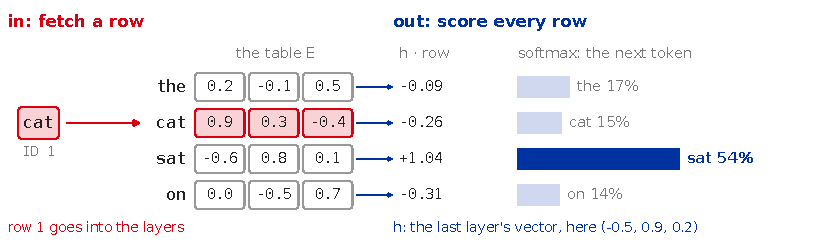
\includegraphics[width=0.92\linewidth]{emb_unembed.pdf}\end{center}
  \vskip -8pt
  {\footnotesize The toy table from the lookup slide. ``sat'' wins: its row gives the largest dot
  product with $h$, $(-0.5)(-0.6) + (0.9)(0.8) + (0.2)(0.1) = 1.04$.}
\end{frame}

\begin{frame}{Who ties, and why}
  \begin{itemize}
    \item The output step is often called the \textbf{unembedding}, or the language-model head (LM
      head, the map's name for it).
    \item Small models tie, big ones usually keep two tables, one for each job. Tied: Qwen3-0.6B
      (2025), Gemma 4 E2B (2026). Not tied: Qwen3-8B (2025), gpt-oss-20b (2025), DeepSeek-V3
      (2024).
  \end{itemize}
  \vskip 10pt
  \takebox{Sharing works because both jobs want the same thing: tokens used alike get vectors
  alike. Why the split: in a small model the table is a quarter or more of all parameters (the
  GPT-2 slide), so sharing it saves a lot. In a big one it is a few percent.}
  \vskip 4pt
  \src{\texttt{tie\_word\_embeddings} in each model's config.json, checked 4 Oct 2026.}
\end{frame}

% ============================================================ 2. WHERE IS THE ORDER
\section{Where is the order?}
\sectiontransition{Where is the order?}{A table lookup has no idea where the token sat.}

\begin{frame}{Back to the dog}
  \begin{itemize}
    \item `` dog'' is the 2nd token of ``The dog bites the man'' and the 5th of ``The man bites
      the dog''. The table hands back the same row both times.
    \item So after the lookup, each sentence is just \textbf{five vectors}, and they are the same
      five. The model has received a \textbf{set}: which vectors, but not in what order.
    \item ``Dog bites man'' is not news. ``Man bites dog'' is. The difference is entirely in the
      order.
  \end{itemize}
  \vskip 10pt
  \keybox{Writing the vectors in a list on the slide gives them an order. The question is
  whether anything \textbf{inside the model} can tell which one was first.}
\end{frame}

\begin{frame}{Why the next layer cannot recover it}
  \small
  A preview of LLM-3. The next layer updates each vector like this:
  \begin{enumerate}
    \item compare it with every other vector: a \textbf{dot product} of their numbers;
    \item turn those scores into weights;
    \item add the vectors up with those weights.
  \end{enumerate}
  \vskip 4pt
  Each step uses only \textbf{what is in} the vectors. None of them reads a slot number, and a
  weighted sum gives the same total whatever order you add in. Next slide: by hand. The
  attention lecture proves it in general: shuffle the inputs and every output comes back
  unchanged, just shuffled.
  \vskip 8pt
  \keybox{An RNN never had this problem: it read tokens one at a time, so order was built into
  the computation ([53]). Attention reads all tokens at once - that is why it is fast - and the
  price is that order is gone.}
\end{frame}

\begin{frame}{By hand: shuffle the sentence, and nothing changes}
  \small
  Toy vectors with 2 numbers: dog $= (1, 0)$, bites $= (1, 1)$, man $= (0, 1)$. The next layer,
  simplified (LLM-3 adds learned matrices), updates ``dog'':
  \vskip 2pt
  \begin{center}
  \begin{tabular}{l|lcc|lcc}
    & \multicolumn{3}{c|}{\textbf{dog bites man}} & \multicolumn{3}{c}{\textbf{man bites dog}} \\
    slot & vector & score & weight & vector & score & weight \\
    \hline
    0 & dog $(1, 0)$ & 1 & 0.42 & man $(0, 1)$ & 0 & 0.16 \\
    1 & bites $(1, 1)$ & 1 & 0.42 & bites $(1, 1)$ & 1 & 0.42 \\
    2 & man $(0, 1)$ & 0 & 0.16 & dog $(1, 0)$ & 1 & 0.42 \\
  \end{tabular}
  \end{center}
  \vskip 2pt
  \begin{enumerate}
    \item Score: the dot product with dog's vector. dog $\cdot$ bites $= 1 \cdot 1 + 0 \cdot 1 = 1$.
    \item Weight: softmax of the scores, as in multiclass classification: $e^1, e^1, e^0$
      divided by their sum gives $0.42, 0.42, 0.16$.
    \item Output: $0.42 \cdot (1, 0) + 0.42 \cdot (1, 1) + 0.16 \cdot (0, 1) =
      \mathbf{(0.84,\; 0.58)}$ - in \textbf{both} sentences.
  \end{enumerate}
  \vskip 2pt
  \keybox{Each weight travels with its vector, not with its slot. Shuffling the sentence only
  shuffles the rows of this table.}
\end{frame}

\begin{frame}{The fix: write the slot into the vector}
  \small
  Give every \textbf{slot} its own vector too, and add it to the token's row:
  \[
    \text{input}_i \;=\; \underbrace{E[\text{token}_i]}_{\text{which token}}
      \;+\; \underbrace{P[i]}_{\text{which slot}}
  \]
  \begin{center}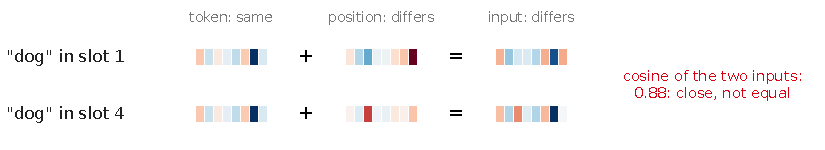
\includegraphics[width=\linewidth]{emb_add_position.pdf}\end{center}
  \vskip -4pt
  Now ``dog in slot 1'' and ``dog in slot 4'' are different inputs, and anything that compares
  vectors can tell them apart. Real GPT-2 rows above: the first 8 of 768 numbers.
\end{frame}

\begin{frame}{By hand: add positions, and dog's output changes}
  \small
  Same toy, plus a vector per slot: slot 0 $= (0.5, 0)$, slot 1 $= (0, 0)$, slot 2 $= (0, 0.5)$.
  Add them, then run the same three steps for ``dog'':
  \vskip 2pt
  \begin{center}
  \begin{tabular}{l|lcc|lcc}
    & \multicolumn{3}{c|}{\textbf{dog bites man}} & \multicolumn{3}{c}{\textbf{man bites dog}} \\
    slot & input & score & weight & input & score & weight \\
    \hline
    0 & dog $(1.5, 0)$ & 2.25 & 0.63 & man $(0.5, 1)$ & 1.00 & 0.25 \\
    1 & bites $(1, 1)$ & 1.50 & 0.30 & bites $(1, 1)$ & 1.50 & 0.42 \\
    2 & man $(0, 1.5)$ & 0 & 0.07 & dog $(1, 0.5)$ & 1.25 & 0.33 \\
    \hline
    & \multicolumn{3}{l|}{dog's output: $\mathbf{(1.25,\; 0.40)}$} &
      \multicolumn{3}{l}{dog's output: $\mathbf{(0.87,\; 0.84)}$} \\
  \end{tabular}
  \end{center}
  \vskip 4pt
  ``dog'' is now a different vector in each sentence ($(1.5, 0)$ in slot 0, $(1, 0.5)$ in slot
  2), so every score changes, so the weights and the output change.
  \vskip 6pt
  \takebox{Same words, different outputs: the layer can now tell who bit whom. Yet the three
  inputs still add up to $(2.5, 2.5)$ in both sentences. That is the trap on the next slide.}
\end{frame}

\begin{frame}{Trap: adding positions does not fix a sum}
  \vskip 4pt
  Take the cold open again, with position vectors added this time, and add up the five inputs:
  \[
    \sum_i \big(E[\text{token}_i] + P[i]\big) \;=\; \sum_i E[\text{token}_i] \;+\; \sum_i P[i]
  \]
  Both sentences have the same tokens and the same five slots, so both sums are the same. We
  measured it on GPT-2: the two totals still agree to the last bit. The toy said the same:
  $(2.5, 2.5)$ twice.
  \vskip 10pt
  \trapbox{Positions do not change the \textbf{total}; they change \textbf{each vector}. That is
  enough, because the next layer compares vectors pair by pair before it adds anything up (last
  slide: dog's output moved from $(1.25, 0.40)$ to $(0.87, 0.84)$). A model that only summed or
  averaged its inputs would stay blind to order.}
\end{frame}

% ============================================================ 3. LEARNED POSITIONS
\section{Option 1: learn the positions}
\sectiontransition{Option 1: learn the positions}{Another table, one row per slot.}

\begin{frame}{GPT-2's position table}
  \begin{itemize}
    \item A second table, $P$: one row per slot, 768 numbers per row, trained by
      backpropagation exactly like the token table.
    \item It has \textbf{1,024} rows: 786,432 numbers, 0.63\% of GPT-2. Cheap.
    \item Slot 1,025 has no row. GPT-2 cannot read a 1,025th token at all: the limit is built
      into the shape of a matrix. This limit is the model's \textbf{context length}: the most
      tokens it can read at once.
    \item BERT (2018) did the same with 512 rows. Longer documents had to be cut into pieces.
  \end{itemize}
  \vskip 10pt
  \keybox{Nobody told GPT-2 that slot 7 comes between slots 6 and 8. To the training
  procedure they are 1,024 unrelated rows.}
\end{frame}

\begin{frame}{Predict first}
  \vskip 30pt
  \begin{center}
    {\Large\color{popblue}\textbf{After training, what do those 1,024 rows look like?}}
    \vskip 14pt
    {\small Random noise? Something smooth? Something else?}
    \vskip 24pt
    {\small\color{gray}Commit to an answer.}
  \end{center}
\end{frame}

\begin{frame}{It learned waves on its own}
  \begin{center}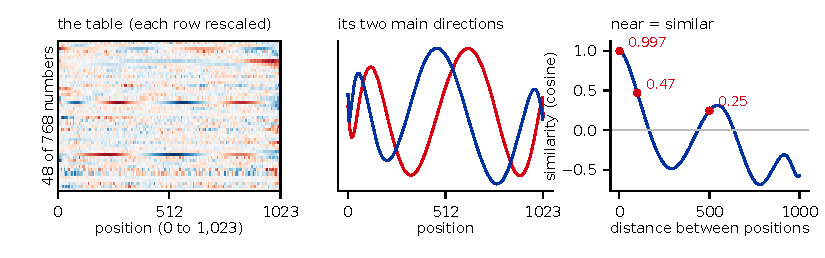
\includegraphics[width=\linewidth]{emb_gpt2_positions.pdf}\end{center}
  \vskip 2pt
  {\small Three views of the same 1,024 rows: the raw numbers (left), a two-number summary of each
  row (middle), and how alike two rows are by distance (right). One at a time, next.}
\end{frame}

% the three panels of emb_gpt2_positions.pdf, cropped (GPT-2's weights are no longer in the HF
% cache, so the figure cannot be redrawn as three). Trims in bp, edges measured at 200 dpi: the
% middle panel's curves end at x = 3.62 in, the right panel's y label spans 3.625-3.715 in above
% y = 0.40 in, the middle panel's "1023" tick label sits below y = 0.36 in.
\begin{frame}{View 1: the table itself}
  \begin{columns}[T]
    \column{0.47\textwidth}
    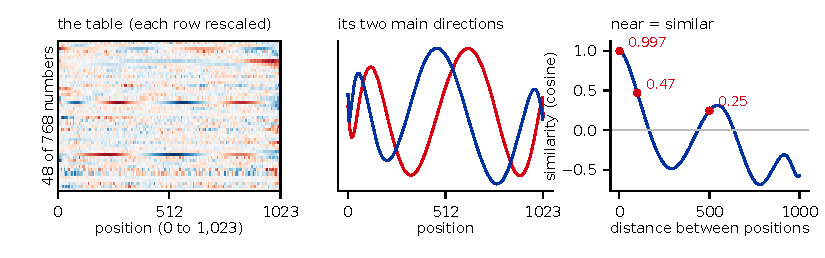
\includegraphics[width=\linewidth,trim=0 0 248 0,clip]{emb_gpt2_positions.pdf}
    \column{0.51\textwidth}
    \small
    \begin{itemize}
      \item Each \textbf{column} is one slot: its row of numbers, stood on end. Slot 0 on the
        left, slot 1,023 on the right.
      \item Only 48 of the 768 numbers fit. Red is positive, blue negative. Each number is
        stretched to its own range, so the faint ones show too.
      \item Read one \textbf{horizontal line}: the same number, slot after slot. It rises and
        falls slowly, in long bands.
    \end{itemize}
  \end{columns}
  \vskip 10pt
  \keybox{Neighbouring columns look almost the same. The rows started as random noise, and
  nothing in training said that slot 7 sits between 6 and 8. Training made them smooth anyway.}
\end{frame}

\begin{frame}{View 2: two numbers summarise each row}
  \begin{columns}[T]
    \column{0.34\textwidth}
    \gptpanel{\linewidth}{155 0 127 0}{0.928}{0.233}{1.01}{1.01}
    \column{0.64\textwidth}
    \small
    \begin{itemize}
      \item 768 numbers per row are too many to plot. PCA (ch10) finds the few
        \textbf{directions} in which the 1,024 rows differ most.
      \item Three directions hold 90\% of the differences, so each row is roughly
        \[\text{average row} + a \cdot \text{dir}_1 + b \cdot \text{dir}_2 + c \cdot \text{dir}_3 .\]
      \item The plot shows $a$ (red) and $b$ (blue) for every slot: how much of direction 1 and
        of direction 2 that slot's row contains.
    \end{itemize}
  \end{columns}
  \vskip 8pt
  \keybox{Both are slow waves, a few swings across the 1,024 slots, with blue running about a
  quarter-swing ahead of red. That is what a turning clock hand looks like from two sides, a
  sine and a cosine. Option 2 builds exactly this on purpose.}
\end{frame}

\begin{frame}{View 3: how alike are two slots, by distance?}
  \begin{columns}[T]
    \column{0.40\textwidth}
    \begin{tikzpicture}   % two masks: the middle panel's "1023" label and its last tick mark
      \node[anchor=south west, inner sep=0] (im)
        {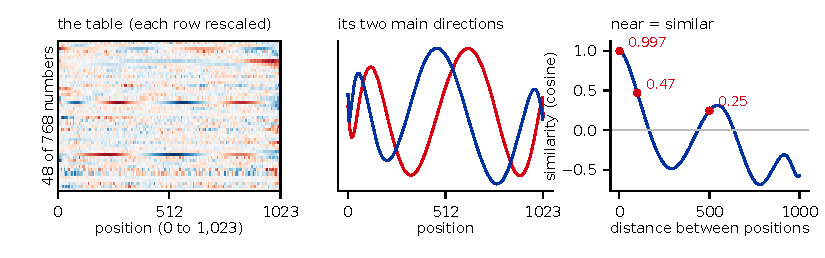
\includegraphics[width=\linewidth,trim=261 0 0 0,clip]{emb_gpt2_positions.pdf}};
      \begin{scope}[x={(im.south east)}, y={(im.north west)}]
        \fill[white] (-0.01,-0.01) rectangle (0.065,0.233);
        \fill[white] (-0.01,0.2) rectangle (0.012,0.262);
      \end{scope}
    \end{tikzpicture}
    \column{0.58\textwidth}
    \small
    Pick two slots $k$ apart, take the cosine of their two rows, and average over every such
    pair of slots. Plot that against $k$.
    \begin{itemize}
      \item $k = 1$: \textbf{0.997}. Neighbours are almost the same row.
      \item $k = 100$: 0.47. $k = 500$: 0.25.
      \item In between it goes \textbf{below zero}: roughly 150 to 450 slots apart, and again
        past about 650.
    \end{itemize}
  \end{columns}
  \vskip 8pt
  \keybox{Near slots look alike, far slots less so. But ``less'' is not steady: the curve swings
  up and down. Next: what a negative cosine means.}
\end{frame}

\begin{frame}{Why the similarity goes below zero}
  \begin{center}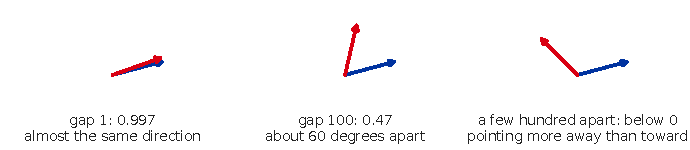
\includegraphics[width=0.84\linewidth]{emb_cos_sign.pdf}\end{center}
  \vskip -2pt
  \small
  \begin{itemize}
    \item A cosine is an angle: $+1$ same direction, $0$ perpendicular, $-1$ opposite. Below zero,
      the two rows point more \textbf{away} from each other than toward.
    \item View 2: each row is mostly ``where its slot sits on the waves''. Those waves take a few
      hundred slots per swing. Two slots half a swing apart sit on opposite sides, one near a
      crest, the other near a trough: their wave parts have opposite signs, so the rows point
      roughly opposite ways.
    \item A full swing apart they are back in step, and the curve climbs again.
  \end{itemize}
  \vskip 2pt
  \takebox{Order was learned from scratch, smooth and wave-like. Remember that for option 2: its
  formula dips below zero for exactly this reason.}
\end{frame}

\begin{frame}{Learned positions: the bill}
  \begin{itemize}
    \item \textbf{A hard length limit.} The table has as many rows as the longest training text,
      and no row exists beyond it.
    \item \textbf{Nothing carries over.} Slot 2,000 cannot be guessed from slots 1 to 1,024: a
      new row needs training data at that length.
    \item \textbf{Absolute, not relative.} ``Three slots back'' has to be learned separately for
      slot 10, slot 500 and slot 1,000. Nothing in the setup says they are the same idea.
  \end{itemize}
  \vskip 10pt
  \keybox{The waves on the last slides suggest a cheaper route: if smooth waves are what the
  model wants, write them down instead of learning them.}
\end{frame}

\begin{frame}{Are the last slots trained less often?}
  \begin{center}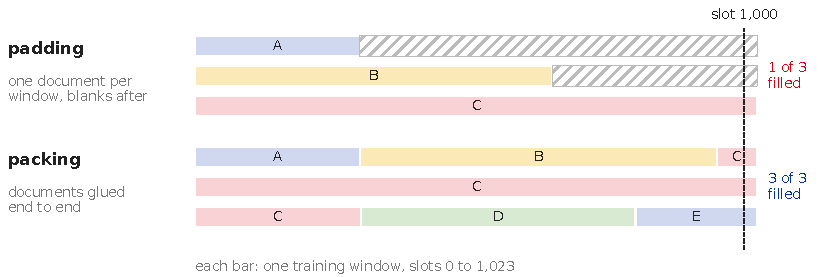
\includegraphics[width=\linewidth]{emb_pack_pad.pdf}\end{center}
  \vskip -4pt
  \small
  It depends on how the training text is cut into 1,024-token windows.
  \begin{itemize}
    \item \textbf{Padding}: one document per window, blanks after it. Then \textbf{yes}: slot
      1,000 only trains on documents longer than 1,000 tokens, and most are shorter.
    \item \textbf{Packing}: documents glued end to end, cut into full windows. Then \textbf{no}:
      every slot is filled in every window, so slot 1,000 trains as often as slot 10.
  \end{itemize}
\end{frame}

\begin{frame}{Two real recipes}
  \begin{itemize}
    \item \textbf{BERT (2018)} made the last slots rare on purpose: 90\% of its training steps used
      128-token windows, the last 10\% used 512, ``to learn the positional embeddings''. Rows 128
      to 511 of its position table trained in a tenth of the steps. Long windows cost more
      (attention compares every pair), so it saved them for the end.
    \item \textbf{GPT-3 (2020)} packs: it ``always'' trains on full 2,048-token windows, documents
      glued together with an end-of-text token between them. Every slot gets its share.
  \end{itemize}
  \vskip 10pt
  \keybox{With packing, the last slots are fine. What stays rare is a long \textbf{gap} inside one
  document. More on that in the last section.}
  \vskip 4pt
  \src{Devlin et al. (2018), BERT, appendix A.2. Brown et al. (2020), GPT-3, section 2.3.}
\end{frame}

% ============================================================ 4. SINUSOIDS
\section{Option 2: write the positions down}
\sectiontransition{Option 2: write the positions down}{No training, and a value for every slot.}

\begin{frame}{A clock with many hands}
  \small
  The original Transformer (Vaswani et al., 2017) fixes $P$ with a formula. For slot $pos$ and
  dimension pair $i$ (of $d$ dimensions):
  \[
    P_{pos,\,2i} = \sin\!\left(\frac{pos}{10000^{2i/d}}\right) \qquad
    P_{pos,\,2i+1} = \cos\!\left(\frac{pos}{10000^{2i/d}}\right)
  \]
  \vskip -4pt
  \begin{center}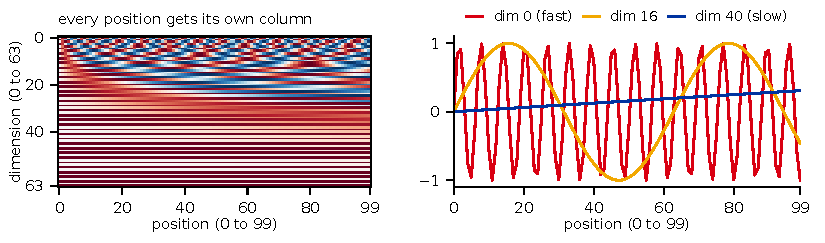
\includegraphics[width=\linewidth]{emb_sinusoid_heatmap.pdf}\end{center}
  \vskip -6pt
  Each pair of dimensions is a clock hand turning at its own speed. Fast hands tell neighbours
  apart; slow hands tell far-apart slots apart. Together they give every slot a unique reading.
  (Here $d = 64$, slots 0 to 99; the next plot uses $d = 128$.)
\end{frame}

\begin{frame}{Similarity depends on the gap only}
  \begin{columns}[T]
    \begin{column}{0.60\textwidth}
      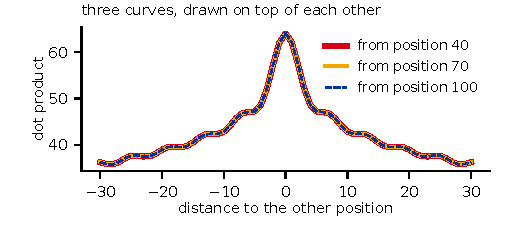
\includegraphics[width=\linewidth]{emb_sinusoid_gap.pdf}
    \end{column}
    \begin{column}{0.38\textwidth}
      \small
      The dot product of two slots' vectors, starting from slots 40, 70 and 100: the three curves
      are \textbf{identical} (largest difference below $10^{-9}$). Only the distance matters,
      not where you are.
    \end{column}
  \end{columns}
  \vskip 6pt
  \keybox{So for the bare waves, ``three slots back'' looks the same at slot 10 and at slot 1,000.
  Inside a real model it gets messier (option 3 says why).}
  \vskip 4pt
  \trapbox{The formula has a value for every slot, so it seems to promise texts longer than any
  seen in training. In practice it does not deliver: trained on 512 or 1,024 tokens, such
  models get worse soon after the training length (Press et al., 2022). The model never learned
  to use the unseen readings.}
\end{frame}

\begin{frame}{Why compare two slots? One clock hand, by hand}
  \small
  \begin{itemize}
    \item The next layer compares vectors with dot products (the shuffle toy). So what position
      contributes is how two slots' vectors compare: $P_a \cdot P_b$. We want that to depend on how
      \textbf{far apart} $a$ and $b$ are, nothing else.
    \item Take a single pair of dimensions turning $30^\circ$ per slot. Slot $a$ holds
      $(\sin 30a^\circ,\; \cos 30a^\circ)$: an arrow of length 1, turned $30a^\circ$.
  \end{itemize}
  \vskip 2pt
  \begin{center}
  \begin{tabular}{llll}
    \textbf{slots} & \textbf{angles} & \textbf{vectors} & \textbf{dot product} \\ \hline
    1 and 3 & $30^\circ$, $90^\circ$ & $(0.5,\; 0.87) \cdot (1,\; 0)$ & $0.5 + 0 = \mathbf{0.5}$ \\
    6 and 8 & $180^\circ$, $240^\circ$ & $(0,\; -1) \cdot (-0.87,\; -0.5)$ & $0 + 0.5 = \mathbf{0.5}$ \\
  \end{tabular}
  \end{center}
  \vskip 2pt
  Both pairs are 2 slots apart, so their arrows are $60^\circ$ apart, and $\cos 60^\circ = 0.5$.
  \vskip 6pt
  \keybox{For arrows of length 1, the dot product is the cosine of the angle between them. In
  symbols, with speed $\omega$: $\sin(\omega a)\sin(\omega b) + \cos(\omega a)\cos(\omega b) =
  \cos\big(\omega (a - b)\big)$. Only the gap is left.}
\end{frame}

\begin{frame}{Why one hand is not enough}
  \begin{center}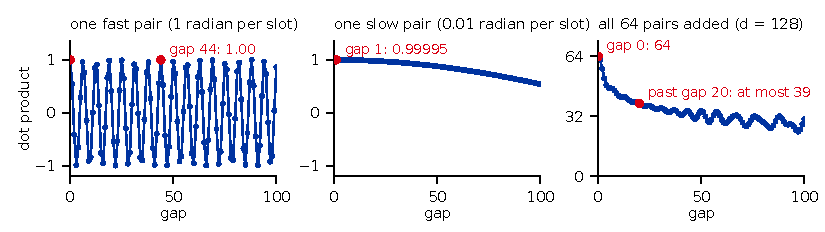
\includegraphics[width=0.88\linewidth]{emb_one_pair.pdf}\end{center}
  \vskip -4pt
  \small
  \begin{itemize}
    \item A \textbf{fast} hand alone repeats: in 44 slots it turns 7 times round, so gap 44 scores
      1.00, like gap 0. It cannot tell near from far.
    \item A \textbf{slow} hand alone barely moves: gap 1 scores 0.99995. It cannot tell neighbours
      apart.
    \item All 64 hands added: only gap 0 reaches 64. Gap 1 still scores 62 (neighbours alike), and
      gaps 20 to 100 stay at 39 or below.
  \end{itemize}
  \vskip 0pt
  \keybox{Like a clock: the seconds hand tells neighbouring moments apart, the hour hand far-apart
  ones. That is why there are many pairs.}
\end{frame}

\begin{frame}{All the hands together: only the gap is left}
  \small
  Pair $i$ turns at its own speed $\omega_i$ and adds $\cos\big(\omega_i (a - b)\big)$ to the dot
  product (two slides back). Add up all $d/2$ pairs:
  \[
    P_a \cdot P_b \;=\; \sum_{i} \cos\big(\omega_i\,(a - b)\big),
    \qquad \omega_i = \frac{1}{10000^{2i/d}}
  \]
  \vskip -2pt
  \begin{itemize}
    \item Only $a - b$ is left: the address cancels. That is why the three curves were one.
    \item At gap 0 every term is $\cos 0 = 1$, so the dot product peaks at $d/2$: 64 in the plot,
      where $d = 128$.
    \item Further apart, the pairs turn at different speeds and drift out of step; their terms
      partly cancel. Those are the wobbles.
  \end{itemize}
  \vskip 4pt
  \keybox{Hold on to $\cos(\omega(a - b))$: RoPE (option 3) is built on exactly this identity.}
\end{frame}

\begin{frame}{Predict first}
  \vskip 26pt
  \begin{center}
    {\Large\color{popblue}\textbf{Every model here \emph{adds} the position vector\\ to the token
    vector. Why not put them side by side?}}
    \vskip 14pt
    {\small Adding mixes two kinds of information into the same 768 numbers. Surely that blurs
    the token?}
    \vskip 24pt
    {\small\color{gray}Commit to an answer.}
  \end{center}
\end{frame}

\begin{frame}{By hand: adding can be concatenation in disguise}
  \small
  A toy with 4 numbers per vector. Tokens use the first two, slots the last two:
  \[
    \text{dog} = (3, 1, 0, 0) \quad \text{cat} = (1, 3, 0, 0) \qquad
    \text{slot 1} = (0, 0, 1, 0) \quad \text{slot 4} = (0, 0, 0, 1)
  \]
  \[
    \text{dog in slot 4} = (3, 1, 0, 0) + (0, 0, 0, 1) = (3, 1, 0, 1)
  \]
  \begin{itemize}
    \item The first two numbers still say ``dog'': the dot product with dog is
      $3 \cdot 3 + 1 \cdot 1 = 10$, with cat only $3 \cdot 1 + 1 \cdot 3 = 6$.
    \item The last two numbers say ``slot 4''. Nothing was blurred.
    \item Putting them side by side, $(3, 1 \,|\, 0, 1)$, is the same thing, except that every
      later layer must be wider to accept the longer vector.
  \end{itemize}
  \vskip 4pt
  \keybox{If tokens and slots live in \textbf{different directions}, adding them loses nothing.
  The question is whether a real model keeps them apart.}
\end{frame}

\begin{frame}{Side by side has a price}
  \small
  Three ways to give a 768-number token a 768-number position:
  \begin{itemize}
    \item \textbf{Side by side, 1,536 numbers.} Every weight matrix in every layer grows on both
      sides, so each layer gets about 4 times the weights: GPT-2's 12 layers would go from 85M to
      340M parameters.
    \item \textbf{Side by side inside 768}, say 640 for the token and 128 for the slot. No growth,
      but every token starts with 128 fewer numbers of its own.
    \item \textbf{Add.} The token keeps all 768, the slot gets all 768, nothing grows. The catch:
      both share the same numbers.
  \end{itemize}
  \vskip 6pt
  \keybox{And side by side is less different than it looks. The first thing a layer does is
  multiply by a matrix. Cut the matrix into a token part and a slot part:
  $W \begin{pmatrix} e \\ p \end{pmatrix} = W_1 e + W_2 p$. Side by side, then a matrix,
  \textbf{is} adding, just of two transformed vectors.}
\end{frame}

\begin{frame}{First: random directions in 768 dimensions}
  \begin{columns}[T]
    \begin{column}{0.58\textwidth}
      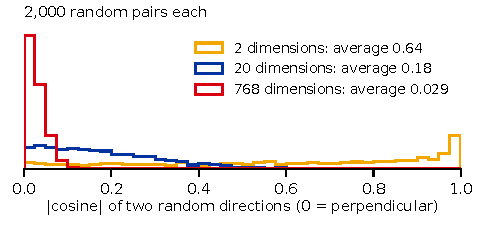
\includegraphics[width=\linewidth]{emb_random_cos.pdf}
    \end{column}
    \begin{column}{0.40\textwidth}
      \small
      Draw two directions at random and take $|\cos|$ of the angle between them: 0 means
      perpendicular, 1 means the same line.
      \vskip 6pt
      In 2 dimensions it can be anything: average 0.64. In 768 dimensions two random directions are
      almost always nearly perpendicular: average 0.029.
    \end{column}
  \end{columns}
  \vskip 10pt
  \keybox{So 768 dimensions leave room for many directions that barely overlap. If token rows and
  slot rows sit in such directions, adding them blurs almost nothing. Does GPT-2 do that? Two
  tests on its real tables.}
\end{frame}

\begin{frame}{Test 1: do GPT-2's token rows and slot rows overlap?}
  \begin{columns}[T]
    \begin{column}{0.62\textwidth}
      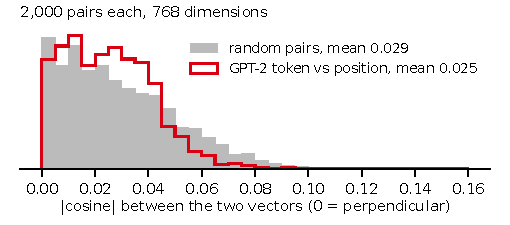
\includegraphics[width=\linewidth]{emb_add_vs_concat.pdf}
    \end{column}
    \begin{column}{0.36\textwidth}
      \small
      Red: 2,000 random pairs (one token row, one slot row) from GPT-2's two tables, $|\cos|$ of
      each pair.
      \vskip 4pt
      Grey: 2,000 pairs of random directions, as on the last slide.
    \end{column}
  \end{columns}
  \vskip 8pt
  \small
  Average $|\cos|$: \textbf{0.025} for GPT-2's pairs, 0.029 for random ones. Token rows and slot
  rows overlap \textbf{no more than random directions do}: they ended up nearly perpendicular.
  \vskip 6pt
  \keybox{Test 1 says the directions barely overlap. Test 2 checks what that buys: after adding,
  is the token still readable?}
\end{frame}

\begin{frame}{Test 2: can we still read the token after adding?}
  \small
  \begin{enumerate}
    \item Pick a random token and a random slot. Add their rows: the input the model really gets.
    \item Ask which of the 50,257 token rows points most the same way as that sum.
    \item Count it as right if that is the token we started from.
  \end{enumerate}
  \vskip 2pt
  The 4-number toy did the same by hand: $(3, 1, 0, 1)$ still scored highest with dog (10, against 6
  for cat).
  \vskip 6pt
  On GPT-2: right \textbf{1,998 times out of 2,000}. The 2 misses: a stray byte and
  `` RandomRedditor'', a glitch token. The barely-trained rows again.
  \vskip 8pt
  \takebox{The answer to the predict slide: adding does not blur the token. 768 dimensions leave
  room for directions that barely overlap, so adding costs nothing and keeps both messages
  readable.}
\end{frame}

% ============================================================ 5. ROPE
\section{Option 3: rotate, do not add}
\sectiontransition{Option 3: rotate, do not add}{What a comparison needs is the gap, not the
address.}

\begin{frame}{What attention needs from position}
  \small
  The next layer compares pairs of tokens (LLM-3). From each token's vector it makes two new ones:
  a \textbf{query} (``what am I looking for?'') and a \textbf{key} (``what do I offer?''). The
  score of a pair is query $\cdot$ key, the dot product from the toy.
  \vskip 8pt
  The same five words, once at the start of a text and once deep inside it:
  \vskip 4pt
  \begin{center}
  \begin{tabular}{l|ccccc}
    slots & 1 & 2 & 3 & 4 & 5 \\
    tokens & The & \textcolor{armred}{\textbf{cat}} & then & quietly &
      \textcolor{popblue}{\textbf{sat}} \\
    \hline
    slots & 41 & 42 & 43 & 44 & 45 \\
    tokens & the & \textcolor{armred}{\textbf{cat}} & then & quietly &
      \textcolor{popblue}{\textbf{sat}} \\
  \end{tabular}
  \end{center}
  \vskip 6pt
  ``sat'' looks back for whoever sat: ``cat'', 3 slots earlier, both times. Same words, same gap,
  so the score should be the same. Where the pair sits in the text should not matter.
  \vskip 8pt
  \keybox{\textbf{Predict:} with a position vector \emph{added} to each token (options 1 and 2),
  is the score of ``sat'' looking at ``cat'' the same at slots 5 and 2 as at 45 and 42?}
\end{frame}

\begin{frame}{A toy says no: the address leaks in}
  \begin{columns}[T]
    \begin{column}{0.56\textwidth}
      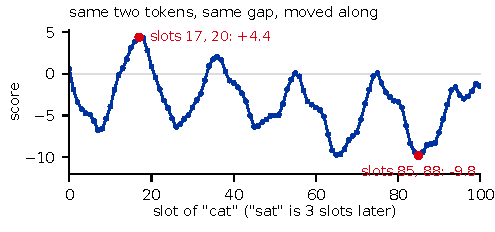
\includegraphics[width=\linewidth]{emb_address_leak.pdf}
    \end{column}
    \begin{column}{0.42\textwidth}
      \small
      A toy layer: 16-number vectors for ``cat'' and ``sat'', random query and key matrices,
      sinusoid positions added to both.
      \vskip 4pt
      Slide the pair along the text, always 3 apart, and score it at every place.
    \end{column}
  \end{columns}
  \vskip 8pt
  \small
  Same two tokens, same gap, and the score swings from \textbf{$-9.8$} to \textbf{$+4.4$} only
  because of \textbf{where} the pair sits. The model would have to learn to undo that.
  \vskip 6pt
  \src{Toy numbers (random vectors, seed 509), not a trained model: the point is that nothing
  stops the address from leaking in. Plot: \texttt{py\_src/embeddings\_position\_figs.py}.}
\end{frame}

\begin{frame}{Why the address leaks in}
  \small
  Write $x = $ token $+$ position, and let $M = W_q^\top W_k$ stand for the two learned matrices.
  The score of ``sat'' in slot $n$ looking at ``cat'' in slot $m$, multiplied out:
  \[
    (e_{\text{sat}} + P_n)^\top M\, (e_{\text{cat}} + P_m) \;=\;
    \underbrace{e_{\text{sat}}^\top M e_{\text{cat}}}_{\text{content}}
    + \underbrace{e_{\text{sat}}^\top M P_m}_{\text{slot } m \text{ alone}}
    + \underbrace{P_n^\top M e_{\text{cat}}}_{\text{slot } n \text{ alone}}
    + \underbrace{P_n^\top M P_m}_{\text{both slots}}
  \]
  \begin{itemize}
    \item The two middle terms each depend on \textbf{one} slot: the address, not the gap.
    \item Even the last term depends on the gap alone only when $M$ is the identity matrix (bare
      waves: the $\cos(\omega(a - b))$ result a few slides back), not after learned matrices.
  \end{itemize}
  \vskip 6pt
  \keybox{Better: build the comparison so that \textbf{only the gap can affect it}. Rotary
  Position Embedding (RoPE; Su et al., 2021): instead of adding a position vector,
  \textbf{rotate} the query and the key by an angle proportional to their slot.}
\end{frame}

\begin{frame}{RoPE, step 1: cut the vector into pairs}
  \begin{center}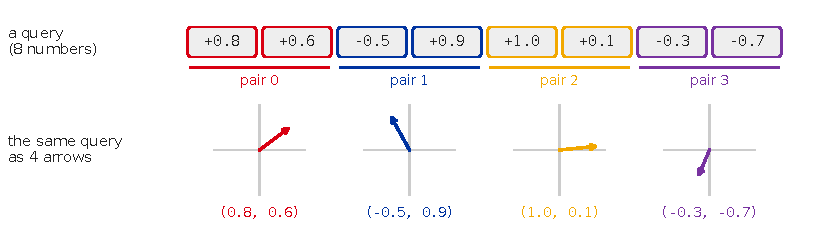
\includegraphics[width=\linewidth]{emb_rope_split.pdf}\end{center}
  \vskip -2pt
  \small
  \begin{itemize}
    \item Numbers 1 and 2 form pair 0, numbers 3 and 4 form pair 1, and so on. Each pair is a
      point in 2-D: draw it as an arrow from the centre.
    \item A real query or key has 128 numbers: \textbf{64 arrows}. Nothing is added or lost: the
      arrows are just another way to look at the same numbers.
  \end{itemize}
  \vskip 4pt
  \src{RoFormer (2021) pairs neighbouring numbers, as here. Llama's code pairs number $i$ with
  number $i + 64$ instead: the same turns, different bookkeeping.}
\end{frame}

\begin{frame}{RoPE, step 2: turn each arrow by its slot}
  \begin{center}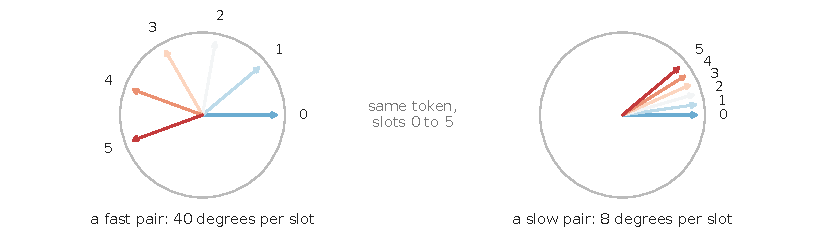
\includegraphics[width=\linewidth]{emb_rope_clock.pdf}\end{center}
  \vskip -4pt
  \small
  \begin{itemize}
    \item One pair of the same token, in slots 0 to 5. In slot $m$, a pair with speed $\theta$ is
      turned by $m \times \theta$: the fast pair $40^\circ$ per slot, the slow pair $8^\circ$.
    \item Turning $(x, y)$ by an angle $\varphi$ gives $(x\cos\varphi - y\sin\varphi,\;
      x\sin\varphi + y\cos\varphi)$. Example: $(1, 0)$ turned by $90^\circ$ is $(0, 1)$.
    \item The arrow's length never changes: only its direction carries the slot. That is why we
      call it a clock hand.
  \end{itemize}
\end{frame}

\begin{frame}{RoPE, step 3: every pair has its own speed}
  \begin{columns}[T]
    \begin{column}{0.58\textwidth}
      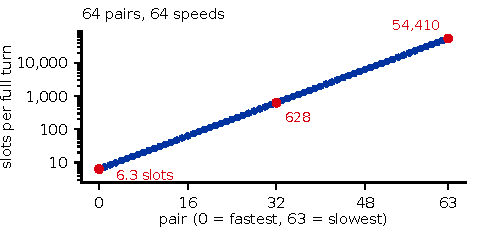
\includegraphics[width=\linewidth]{emb_rope_speeds.pdf}
    \end{column}
    \begin{column}{0.40\textwidth}
      \small
      Pair $i$ turns $\theta_i = 1 / 10000^{2i/d}$ radians per slot: the sinusoids' speeds. With
      128 numbers ($d = 128$), 64 pairs:
      \begin{itemize}
        \item pair 0: 1 radian per slot, a full turn every 6.3 slots;
        \item pair 32: 0.01, every 628;
        \item pair 63: 0.000115, every 54,410.
      \end{itemize}
    \end{column}
  \end{columns}
  \vskip 8pt
  \keybox{Fast hands tell neighbours apart, slow hands tell far-apart slots apart: the clock of
  option 2, but now turning the query and the key themselves.}
\end{frame}

\begin{frame}{Why only the gap survives: the picture}
  \begin{center}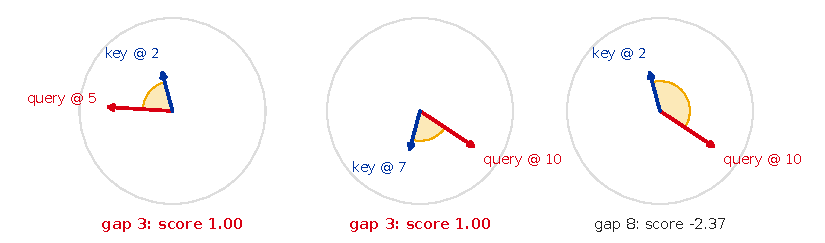
\includegraphics[width=0.86\linewidth]{emb_rope_2d.pdf}\end{center}
  \vskip -6pt
  \small
  \begin{enumerate}
    \item A dot product depends on two lengths and the angle between the arrows:
      $\mathbf{q} \cdot \mathbf{k} = |\mathbf{q}|\,|\mathbf{k}| \cos(\text{angle between})$.
    \item Turn the query by $m\theta$ and the key by $n\theta$. The lengths do not change. The
      angle between them is the unturned angle plus $(m - n)\,\theta$.
    \item So the score depends on the content and the \textbf{gap} $m - n$ only. Left and middle:
      gap 3 at different slots, the same score 1.00. Right: gap 8, another score.
  \end{enumerate}
\end{frame}

\begin{frame}{Why only the gap survives: the algebra}
  \small
  Write a turn by an angle $\varphi$ as a matrix,
  $R(\varphi) = \begin{pmatrix} \cos\varphi & -\sin\varphi \\ \sin\varphi & \cos\varphi \end{pmatrix}$,
  and let $R_m = R(m\theta)$ be the turn in slot $m$.
  \begin{enumerate}
    \item A dot product is a transpose times a vector:
      $(R_m\mathbf{q}) \cdot (R_n\mathbf{k}) = \mathbf{q}^\top R_m^\top R_n\, \mathbf{k}$.
    \item Transposing a turn undoes it: $R_m^\top = R_{-m}$. (Transposing swaps the two sines, and
      $\cos(-x) = \cos x$, $\sin(-x) = -\sin x$.)
    \item Two turns add up: $R_{-m} R_n = R_{n - m}$. Back by $m$, then forward by $n$, is one
      turn by $n - m$.
  \end{enumerate}
  \[
    (R_m\mathbf{q}) \cdot (R_n\mathbf{k}) \;=\; \mathbf{q}^\top R_{n-m}\, \mathbf{k}
  \]
  The slots $m$ and $n$ survive only as $n - m$.
  \vskip 6pt
  \keybox{A real query has 64 pairs, each with its own $\theta_i$. Its score is the \textbf{sum}
  of the 64 pair scores, and each of them depends only on the gap.}
\end{frame}

\begin{frame}{By hand: same gap, same score}
  \small
  $\mathbf{q} = (2, 1)$, $\mathbf{k} = (1, 1)$, $\theta = 30^\circ$ per slot (a toy speed). Unrotated,
  $\mathbf{q} \cdot \mathbf{k} = 2 + 1 = 3$. Turning $(x, y)$ by an angle $\varphi$ gives
  $(x\cos\varphi - y\sin\varphi,\; x\sin\varphi + y\cos\varphi)$.
  \vskip 4pt
  \begin{center}
  \begin{tabular}{llll}
    \textbf{slots} & \textbf{query turned by} & \textbf{key turned by} & \textbf{score} \\
    \hline
    $q$ in 5, $k$ in 2 & $150^\circ$: $(-2.23,\; 0.13)$ & $60^\circ$: $(-0.37,\; 1.37)$ &
      $0.82 + 0.18 = \mathbf{1.00}$ \\
    $q$ in 10, $k$ in 7 & $300^\circ$: $(1.87,\; -1.23)$ & $210^\circ$: $(-0.37,\; -1.37)$ &
      $-0.68 + 1.68 = \mathbf{1.00}$ \\
    $q$ in 10, $k$ in 2 & $300^\circ$: $(1.87,\; -1.23)$ & $60^\circ$: $(-0.37,\; 1.37)$ &
      $-2.37$ \\
  \end{tabular}
  \end{center}
  \vskip 6pt
  Gap 3 gives 1.00 at slots 5/2 and at 10/7. Gap 8 gives something else. Swap the roles ($q$ in
  2, $k$ in 5: gap $-3$) and it is $-1.00$: the gap is signed, so before and after differ. Check one row
  yourself: $\cos 150^\circ = -0.866$, $\sin 150^\circ = 0.5$, so the query becomes
  $(2 \cdot (-0.866) - 1 \cdot 0.5,\; 2 \cdot 0.5 + 1 \cdot (-0.866)) = (-2.23,\; 0.13)$.
  \vskip 6pt
  \takebox{The model never sees the slot numbers 5, 2, 10 or 7. It only ever feels the gap.}
\end{frame}

\begin{frame}{By hand: four numbers, two speeds}
  \small
  Two pairs: $\mathbf{q} = \mathbf{k} = (1, 0 \,|\, 1, 0)$. The fast pair turns $90^\circ$ per
  slot, the slow pair $30^\circ$. Each pair's arrows have length 1, so its score is the cosine of
  the angle between them, and the total score is the sum of the two:
  \vskip 2pt
  \begin{center}
  \begin{tabular}{rlll}
    \textbf{gap} & \textbf{fast pair} ($90^\circ$) & \textbf{slow pair} ($30^\circ$) &
      \textbf{score} \\ \hline
    0 & $\cos 0^\circ = 1$ & $\cos 0^\circ = 1$ & $\mathbf{2}$ \\
    1 & $\cos 90^\circ = 0$ & $\cos 30^\circ = 0.87$ & $0.87$ \\
    2 & $\cos 180^\circ = -1$ & $\cos 60^\circ = 0.5$ & $-0.5$ \\
    4 & $\cos 360^\circ = 1$ & $\cos 120^\circ = -0.5$ & $0.5$ \\
  \end{tabular}
  \end{center}
  \vskip 2pt
  Check gap 4 by turning both, $\mathbf{q}$ in slot 5 and $\mathbf{k}$ in slot 1. Fast pair: $(0, 1)
  \cdot (0, 1) = 1$. Slow pair: $(-0.866, 0.5) \cdot (0.866, 0.5) = -0.75 + 0.25 = -0.5$. Total
  0.5, and slots 9 and 5 give 0.5 again.
  \vskip 4pt
  \takebox{The fast pair alone cannot tell gap 4 from gap 0: one full turn looks like no turn.
  The slow pair can. That is why RoPE mixes many speeds, from 1 radian per slot down to 0.000115.}
\end{frame}

\begin{frame}{Back to cat and sat}
  \begin{columns}[T]
    \begin{column}{0.56\textwidth}
      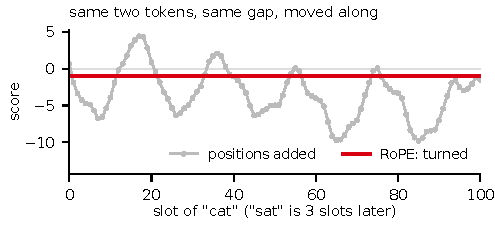
\includegraphics[width=\linewidth]{emb_address_leak_rope.pdf}
    \end{column}
    \begin{column}{0.42\textwidth}
      \small
      The toy from ``the address leaks in'': same vectors, same matrices. Only one change:
      instead of adding positions, turn the query by its slot and the key by its slot.
      \vskip 4pt
      Red: the score is now \textbf{one number} wherever the pair sits (equal to $10^{-9}$).
    \end{column}
  \end{columns}
  \vskip 10pt
  \takebox{The address no longer leaks in: only the gap is left. That is the whole point of
  turning instead of adding.}
\end{frame}

\begin{frame}{Where the rotation happens}
  \begin{center}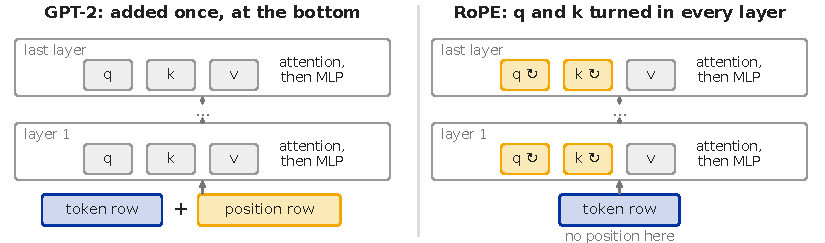
\includegraphics[width=\linewidth]{emb_rope_where.pdf}\end{center}
  \vskip -8pt
  \small
  \begin{itemize}
    \item GPT-2 (left): the position row is added \textbf{once}, at the bottom, and carried up
      through all 12 layers.
    \item RoPE (right): no position at the input. In every layer, each token's query and key are
      turned by its slot right before their dot product; the value $v$ is not turned.
  \end{itemize}
  \vskip 0pt
  \keybox{So position enters every layer's comparison directly. On the map, the Position box stays
  where it is; with RoPE it acts inside attention.}
\end{frame}

\begin{frame}{Who uses it}
  \begin{itemize}
    \item RoFormer (2021) reported modest gains. Adoption was anything but modest: GPT-J (2021)
      and GPT-NeoX (2022), PaLM (2022), then LLaMA (2023), and after LLaMA nearly every open model.
    \item Every 2024-2026 model in the table at the end of today uses RoPE in some form.
    \item Two reasons it won: the score depends only on the gap, and it adds no parameters at
      all - a rotation has nothing to learn.
  \end{itemize}
  \vskip 10pt
  \watchbox{One thing RoPE does not fix by itself: texts longer than the training ones. That is
  the last section.}
\end{frame}

\begin{frame}{Three options, side by side}
  \footnotesize
  \begin{center}
  \begin{tabular}{>{\raggedright\arraybackslash}p{2.2cm}>{\raggedright\arraybackslash}p{3.3cm}%
                  >{\raggedright\arraybackslash}p{3.3cm}>{\raggedright\arraybackslash}p{3.3cm}}
    & \textbf{learned table} (GPT-2) & \textbf{sinusoids} (2017) & \textbf{RoPE} (2021) \\
    \hline
    what it does & adds a trained row per slot & adds a fixed wave pattern & rotates query and key
      inside attention \\[2pt]
    parameters & one row per slot (786,432 numbers in GPT-2) & none & none \\[2pt]
    ``3 slots apart'' & learned separately at every slot & the same pattern everywhere; the model
      must dig it out & the score sees only the gap \\[2pt]
    past the training length & impossible: no row exists & allowed, but quality drops & allowed,
      but quality drops; can be stretched (next section) \\
  \end{tabular}
  \end{center}
  \vskip 8pt
  \keybox{Each option fixes something in the column before it: sinusoids drop the trained rows
  and make the gap the same everywhere; RoPE makes the gap the \textbf{only} thing a comparison
  can see. None of them, by itself, makes a model good at lengths it never trained on.}
\end{frame}

% ============================================================ 6. LONGER AND LONGER
\section{Longer and longer}
\sectiontransition{Longer and longer}{GPT-2 stopped at 1,024 tokens. Models now take a million -
and do not read all of it equally well.}

\begin{frame}{Which hands saw every angle in training?}
  \watchbox{\textbf{Reminder.} A \textbf{hand} is one pair of numbers in a query or key, drawn as an
  arrow. Its \textbf{speed} is how far it turns per slot. 64 hands, from 1 radian per slot (a full
  turn every 6.3 slots) down to 0.000115 (a full turn every 54,410 slots).}
  \vskip 2pt
  \begin{center}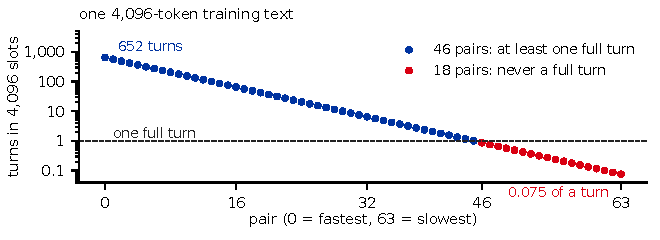
\includegraphics[width=0.80\linewidth]{emb_rope_speeds_train.pdf}\end{center}
  \vskip -4pt
  \small
  A RoPE (2021) model trained on 4,096-token texts, base 10,000, 128-number queries and keys
  (Llama 2's settings, 2023). In one training text the 46 fastest hands go round at least once: they have
  shown the model every angle. The 18 slowest never complete a turn.
\end{frame}

\begin{frame}{Why RoPE breaks past its training length}
  \begin{center}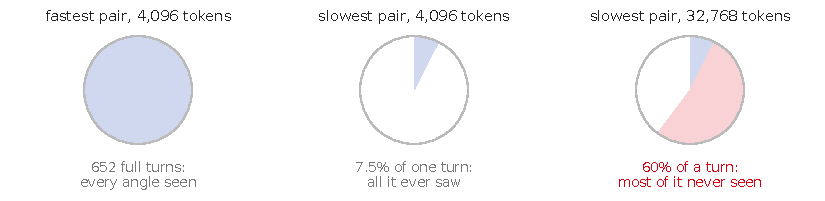
\includegraphics[width=\linewidth]{emb_rope_unseen.pdf}\end{center}
  \vskip -8pt
  \small
  \begin{itemize}
    \item Fastest hand, pair 0 (left): 1 radian per slot, so 4,096 slots make about 650 full
      turns. Every angle seen, many times over.
    \item Slowest hand, pair 63 (middle): $4{,}096 \times 0.000115 = 0.47$ radians, only
      \textbf{7.5\%} of a circle. That thin slice is all the model ever saw of this hand.
    \item Feed it 32,768 tokens (right): the same hand reaches 60\% of its circle. The red part
      holds angles the model never saw, so the scores there are a guess.
  \end{itemize}
  \vskip 2pt
  \src{Press et al. (2022) measured it: RoPE models hold up for 100-200 tokens past their training
  length, then get worse. Sinusoids fail sooner.}
\end{frame}

\begin{frame}{Stretch the clock}
  \begin{itemize}
    \item \textbf{Position interpolation} (Chen et al., 2023): divide every slot number by 8, so
      every hand turns 8 times slower. Slot 32,000 is read as 4,000, an angle the model knows. But
      neighbours now differ by only 1/8 of a step: harder to tell apart.
    \item \textbf{YaRN} (Yet another RoPE extensioN; Peng et al., 2024): slow down only the
      \textbf{slow} hands, the red ones two slides back that never completed a turn. Leave the
      fast hands alone; they have seen every angle anyway.
    \item Then a short extra training run on long documents, so the model gets used to it.
  \end{itemize}
  \vskip 8pt
  \keybox{In 2025 configs: Qwen3-8B (2025), native length 32,768 tokens, reaches 131,072 with YaRN.
  gpt-oss-20b (2025) was stretched from 4,096 to 131,072.}
  \vskip 2pt
  \src{Qwen3-8B model card; gpt-oss-20b config.json (\texttt{rope\_scaling}), checked 4 Oct
  2026.}
\end{frame}

\begin{frame}{Two other answers: a distance penalty, or no position at all}
  \begin{itemize}
    \item \textbf{Attention with Linear Biases} (ALiBi; Press et al., 2022): no position vectors
      at all. Each comparison score just gets a penalty that grows with the distance, so near
      tokens win unless a far one is much more relevant. BLOOM (2022) used it.
    \item \textbf{No Positional Encoding} (NoPE): nothing. A model that may only look back at
      earlier tokens (decoder models, LLM-5) still works out positions on its own (Haviv et al.,
      2022): token 3 sees 3 tokens, token 300 sees 300, and that count gives its position away.
    \item Llama 4 (2025) mixes RoPE and NoPE: some layers rotate, some have no position at
      all. Meta reports up to 10 million tokens of context for Llama 4 Scout.
  \end{itemize}
  \vskip 6pt
  \takebox{Position is still an open design question. The 2017 answer did not last, and the
  2021 answer keeps being patched.}
\end{frame}

\begin{frame}{What models use, 2017-2026}
  \footnotesize
  \begin{center}
  \begin{tabular}{lll}
    \textbf{model} & \textbf{position} & \textbf{context (tokens)} \\
    \hline
    Transformer (2017) & sinusoids & - \\
    BERT (2018) & learned table & 512 \\
    GPT-2 (2019) & learned table & 1,024 \\
    T5 (2019) & a learned bias per distance & 512 in training \\
    BLOOM (2022) & ALiBi & 2,048 \\
    Llama 3.1 (2024) & RoPE, base 500,000, stretched from 8,192 & 131,072 \\
    DeepSeek-V3 (2024) & RoPE + YaRN (from 4,096) & 163,840 \\
    Qwen3-8B (2025) & RoPE, base 1,000,000 & 32,768; 131,072 with YaRN \\
    gpt-oss-20b (2025) & RoPE + YaRN (from 4,096) & 131,072 \\
    Llama 4 Scout (2025) & RoPE layers + NoPE layers & 10,000,000 \\
    Gemma 4 E2B (2026) & RoPE, two bases: 10,000 and 1,000,000 & 131,072 \\
  \end{tabular}
  \end{center}
  \vskip 4pt
  {\small Gemma's two bases: layers that only look at nearby tokens use the faster clock
  (10,000), layers that see the whole text the slower one. Closed models, October 2026: Gemini 4
  Argon 1,048,576 tokens, Claude Opus 5.5 and Fable 5.1 1M, GPT-6 Astra 1,050,000; how they encode
  position is not published.}
  \vskip 2pt
  \src{config.json and model cards on Hugging Face, Meta's Llama 4 announcement, checked 4 Oct
  2026; Llama 3.1's config and the vendors' model pages, checked 27 Oct 2026.}
\end{frame}

\begin{frame}{Why 131,072 and 163,840?}
  \begin{itemize}
    \item $131{,}072 = 2^{17} = 128 \times 1{,}024$: the ``128K'' on the box, counting K as 1,024.
      Llama 3.1 (2024) and Gemma 4 E2B (2026) list it as is.
    \item Stretched models multiply: the length they trained at, times the stretch factor in
      their config.
      \begin{itemize}
        \item DeepSeek-V3 (2024): $4{,}096 \times 40 = \mathbf{163{,}840}$
        \item gpt-oss-20b (2025): $4{,}096 \times 32 = 131{,}072$
        \item Qwen3-8B (2025): $32{,}768 \times 4 = 131{,}072$
      \end{itemize}
    \item Why 40 and not 32? The config does not say.
  \end{itemize}
  \vskip 8pt
  \keybox{Powers of two are a habit and a convenience, not magic: attention code on GPUs usually
  works through the text in blocks of 64 or 128 tokens, and 163,840 $= 1{,}280 \times 128$ divides
  just as evenly.}
  \vskip 2pt
  \src{\texttt{max\_position\_embeddings} and \texttt{rope\_scaling} in each config.json on Hugging
  Face, checked 28 Oct 2026; Qwen3-8B model card.}
\end{frame}

\begin{frame}{Predict first}
  \vskip 26pt
  \begin{center}
    {\Large\color{popblue}\textbf{A question, and 20 documents in the prompt.\\[4pt] One of them
    holds the answer.}}
    \vskip 14pt
    {\small Does it matter whether that document comes first, in the middle, or last?}
    \vskip 24pt
    {\small\color{gray}Commit to an answer.}
  \end{center}
\end{frame}

\begin{frame}{Lost in the middle}
  \begin{columns}[T]
    \column{0.62\textwidth}
    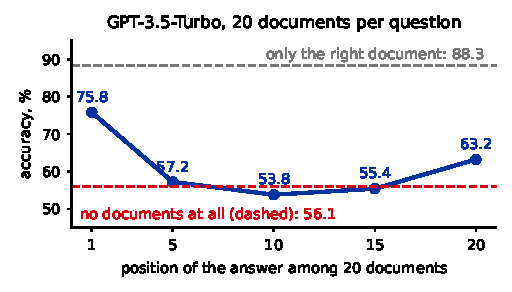
\includegraphics[width=\linewidth]{emb_lost_middle.pdf}
    \column{0.36\textwidth}
    \small
    \vskip 4pt
    A U-shape: the answer is found best at the \textbf{start}, then at the \textbf{end}.
    \vskip 6pt
    In the middle, GPT-3.5 Turbo (2023) does \textbf{worse than with no documents at all} (53.8\%
    vs 56.1\%): there, the extra text actively hurts.
    \vskip 6pt
    The paper measures the effect; it does not settle the cause.
  \end{columns}
  \vskip 6pt
  \keybox{A window that \emph{fits} 20 documents is not a model that \emph{uses} all 20. In a
  long prompt, put what matters first or last.}
  \vskip 2pt
  \src{Liu et al. (2024), ``Lost in the Middle: How Language Models Use Long Contexts'', TACL;
  NaturalQuestions (2019), 20 Wikipedia passages per question; model gpt-3.5-turbo-0613. Plot:
  \texttt{py\_src/long\_context\_figs.py}.}
\end{frame}

\begin{frame}{Claimed length vs used length}
  \begin{itemize}
    \item The classic test hides one sentence, a ``needle'', in a long text and asks for it back.
      Most models now pass it.
    \item \textbf{RULER} (Hsieh et al., 2024): 13 tasks, from several needles at once to tracing a
      variable through a long text and counting frequent words. 17 models, all claiming 32K tokens
      or more: ``only half of them'' hold up at 32K.
    \item \textbf{Context rot} (Chroma, July 2025): 18 models, simple tasks, longer and longer
      inputs. The answers get steadily less reliable as the input grows. Oddly, a shuffled
      haystack was easier than a coherent one.
  \end{itemize}
  \vskip 6pt
  \takebox{Position encoding decides how far a model \emph{can} read. Training decides how well
  it reads that far. Test the length you need; do not trust the number on the box.}
\end{frame}

\begin{frame}{Long gaps are rare in training}
  \begin{columns}[T]
    \begin{column}{0.55\textwidth}
      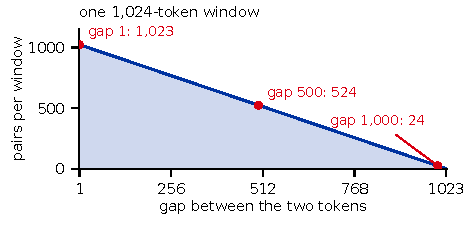
\includegraphics[width=\linewidth]{emb_gap_counts.pdf}
    \end{column}
    \begin{column}{0.43\textwidth}
      \small
      Back to the question from option 1. In one 1,024-token window, two tokens 1 apart occur
      1,023 times, 1,000 apart only 24 times: a window of $L$ tokens holds $L - k$ pairs $k$ apart.
      \vskip 4pt
      And a long gap only teaches something if both tokens sit in the \textbf{same} document.
      Most documents are short; Llama 3 (2024) even blocks attention across document borders in a
      packed window.
    \end{column}
  \end{columns}
  \vskip 6pt
  \small
  So models train short and stretch late. Llama 3 (2024): 8K-token windows for the main run of
  15.6T tokens, then six stages up to 128K, about 800B tokens: roughly 5\% of the training.
  \vskip 4pt
  \takebox{Far-apart pairs get the least practice. That is one likely reason the used length trails
  the claimed one.}
  \vskip 2pt
  \src{Grattafiori et al. (2024), ``The Llama 3 Herd of Models'': the document mask, and long-context
  pre-training of the 405B model.}
\end{frame}

\begin{frame}{The first slots are special: attention sinks}
  \begin{itemize}
    \item Xiao et al. (2024) watched where attention goes in long texts: a large share lands on
      the \textbf{first few tokens}, whatever they say.
    \item Swap the first 4 tokens for line breaks and the model's perplexity (how surprised it is
      by the text; lower is better) barely moves, 5.4 to 5.6. Drop them and keep only a window of
      recent tokens, and it explodes to 5,158. Their position matters, not their meaning.
    \item Why: softmax must hand out weights that sum to 1. When nothing is relevant, the model
      parks the spare attention on a token every later position can see: the first one.
    \item Their fix, StreamingLLM: always keep the first 4 tokens plus a sliding window of recent
      ones. Stable over 4 million tokens.
  \end{itemize}
  \vskip 4pt
  \watchbox{Slot 0 is special in GPT-2's own position table too: its row is about three times
  longer than the median slot's (9.88 vs 3.37), an easy mark for a head to find. LLM-4 measures
  the sinks in GPT-2's heads.}
\end{frame}

% ============================================================ RECAP
\section*{Recap}

\begin{frame}{Recap}
  \begin{itemize}
    \item An ID picks a \textbf{row of a learned table} (one-hot times a matrix). The rows
      learn how tokens are used: days near days, opposites near each other, glitch tokens in a
      pile.
    \item A lookup ignores order: both dog sentences arrive as the same five vectors.
    \item So each vector also gets its \textbf{slot}: a learned row (GPT-2, hard limit 1,024), a
      formula (sinusoids, 2017), or a rotation inside every attention layer (RoPE, 2021: only the
      gap counts).
    \item Adding works because in 768 dimensions token and position directions barely overlap.
    \item Longer texts: stretch the slow clock hands (YaRN, 2024), or penalise distance (ALiBi,
      2022), or drop position in some layers (NoPE, 2022).
    \item Fitting is not using: answers in the middle of a long prompt get lost, claimed lengths
      outrun used ones, and the first tokens soak up spare attention (sinks).
  \end{itemize}
\end{frame}

\begin{frame}{Next on the map}
  \begin{center}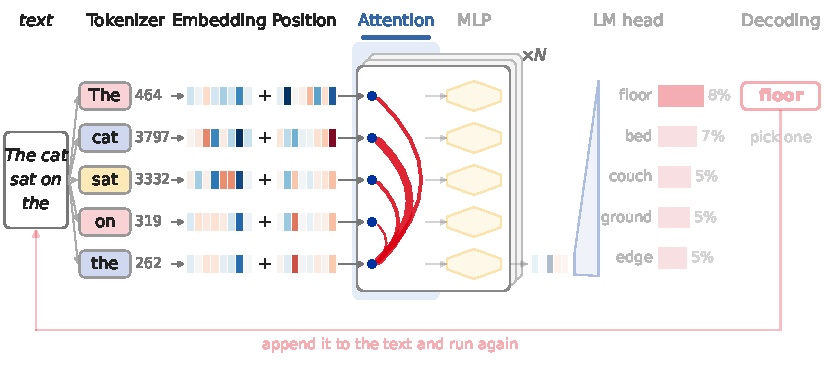
\includegraphics[width=\linewidth]{roadmap_attention_pass.pdf}\end{center}
  \vskip -2pt
  {\small Next (LLM-3): the vectors start talking to each other. (The map is GPT-2, which adds
  position vectors; a RoPE model rotates inside attention instead.)}
\end{frame}

\begin{frame}{Sources \& further reading (1/2)}
  \footnotesize
  \begin{itemize}
    \item \textbf{Watch:} 3Blue1Brown (2024),
      \link{https://youtu.be/wjZofJX0v4M?t=747}{Transformers, the tech behind LLMs \textbar{} Deep
      Learning Chapter 5}; Jia-Bin Huang (2024),
      \link{https://www.youtube.com/watch?v=SMBkImDWOyQ}{How Rotary Position Embedding Supercharges
      Modern LLMs [RoPE]}. \textbf{Play:}
      \link{https://projector.tensorflow.org}{projector.tensorflow.org}.
    \item Vaswani et al. (2017), ``Attention Is All You Need'', NeurIPS (sinusoids).
    \item Su et al. (2021), ``RoFormer: Enhanced Transformer with Rotary Position Embedding'',
      arXiv; Neurocomputing (2024).
    \item Press, Smith \& Lewis (2022), ``Train Short, Test Long: Attention with Linear Biases
      Enables Input Length Extrapolation'', ICLR.
    \item Haviv et al. (2022), ``Transformer Language Models without Positional Encodings Still
      Learn Positional Information'', Findings of EMNLP.
    \item Chen et al. (2023), ``Extending Context Window of Large Language Models via Positional
      Interpolation'', arXiv; Peng et al. (2024), ``YaRN'', ICLR.
    \item Meta (April 2025), ``The Llama 4 herd''; Grattafiori et al. (2024), ``The Llama 3 Herd of
      Models'', arXiv.
  \end{itemize}
  \vskip 2pt
  \src{Every GPT-2 number: \texttt{py\_src/embeddings\_position\_figs.py} (GPT-2's weights read
  with safetensors, IDs from tiktoken), raw results in
  \texttt{results/embeddings\_position\_figs.json}.}
\end{frame}

\begin{frame}{Sources \& further reading (2/2)}
  \footnotesize
  \begin{itemize}
    \item Firth (1957), ``A synopsis of linguistic theory, 1930-1955'', \emph{Studies in
      Linguistic Analysis}.
    \item Mikolov, Yih \& Zweig (2013), ``Linguistic Regularities in Continuous Space Word
      Representations'', NAACL.
    \item Bolukbasi et al. (2016), ``Man is to Computer Programmer as Woman is to Homemaker?
      Debiasing Word Embeddings'', NeurIPS. Nissim, van Noord \& van der Goot (2020), ``Fair is
      Better than Sensational: Man is to Doctor as Woman is to Doctor'', Computational Linguistics.
    \item Land \& Bartolo (2024), ``Fishing for Magikarp'', EMNLP.
    \item Liu et al. (2024), ``Lost in the Middle: How Language Models Use Long Contexts'', TACL.
    \item Hsieh et al. (2024), ``RULER: What's the Real Context Size of Your Long-Context Language
      Models?'', COLM. Hong, Troynikov \& Huber (2025), ``Context Rot'', Chroma technical report.
    \item Xiao et al. (2024), ``Efficient Streaming Language Models with Attention Sinks'', ICLR.
  \end{itemize}
\end{frame}

\end{document}

% ============================================================================
% Provenance:
%   Deck: LLM-2 Embeddings and position (14_llms), session 2 of the LLM chapter (DECISIONS #68).
%   Built 2026-10-04 from LLM2_embeddings_position_OUTLINE.md (instructor interview 2026-10-04:
%   "id like positional encodings to be there, were going left to right") and
%   LLM_CHAPTER_PLAN.md, section 5 (LLM-2).
%   Moved here, not copied: L24's embedding primer ("Recall: a token is a vector", "Directions
%   carry meaning", "Embeddings soak up context") and L25's Position section (5 frames).
%   L24 and L25 were not edited (instructor: reference material until their rework). Ported and
%   adapted: sources/llm_training/16_rope (RoPE paper deck: the clock-hand intuition, "what we
%   actually want", by hand same gap same score, adoption), sources/dl4nlp/02_transformers.tex
%   (position frames), sources/dl4nlp/16_long_context_attention.tex ("Positional encoding for
%   length", "Context window extension").
%   Interview decisions: cold open dog bites man, with the instructor's Kargin Haghordum line
%   (ուրա պարավը, բերեք ատամը քաշեմ) and link; measurements = GPT-2's learned positions and
%   nearest neighbours of more interesting words; long-context tail short, intuition only; by-hand
%   frames = lookup (one-hot x matrix), RoPE, add vs concatenate; word2vec stays in LLM-4.
%   Fixed in the port (L25's sinusoid frames overstated it): sinusoids do NOT extrapolate in
%   practice, and RoPE also degrades past its training length (Press et al. 2022: rotary holds
%   for ~100-200 extra tokens on WikiText-103; YaRN abstract: RoPE models "fail to generalize past
%   the sequence length they were trained on").
%   Figures: fig/emb_*.pdf from py_src/embeddings_position_figs.py (every number quoted in prose
%   asserted in QUOTED; save() refuses any text outside the figure); maps from
%   py_src/llm_roadmap.py (Position stage added for this deck).
%   Measured 2026-10-04 (GPT-2 small, HF cache): the bare phrases are different tokens (dog vs
%   " dog"); "The dog bites the man" / "The man bites the dog" = same 5 IDs, sums identical with
%   and without positions; wte 38,597,376 = 31.0% of 124,439,808; wpe 1,024 rows, 0.63%;
%   learned-position cosine 0.997 (gap 1), 0.47 (100), 0.25 (500), negative in between; top 3
%   directions 90%; slot 0 norm 9.88 vs median 3.37; token vs position |cos| 0.025 (random 0.029);
%   token recovered after adding a position 1998/2000 (misses: a byte token and
%   " RandomRedditor"); dog@1 vs dog@4 input cosine 0.88; analogies (inputs excluded) queen 0.69,
%   actress 0.82, mice 0.70, Armenian 0.79, worse 0.63, Paris fails (Rome 5th), walked fails
%   (swimming); without exclusion 3 of 5 return an input; the 20 rows nearest the mean = 3 glitch
%   names + 17 single-byte tokens; RoPE by hand q=(2,1), k=(1,1), 30 deg: gap 3 -> 1.00 twice,
%   gap 8 -> -2.37, unrotated 3.
%   Verified 2026-10-04 (primary sources): model configs on Hugging Face (BERT 512 absolute;
%   T5 32 relative buckets; Qwen3-8B rope_theta 1e6, 40,960 max, untied; Qwen3-0.6B tied;
%   gpt-oss-20b YaRN 4,096 -> 131,072, untied; DeepSeek-V3 YaRN from 4,096, 163,840, untied;
%   Gemma 4 E2B rope_theta 10,000 sliding / 1,000,000 full, 131,072, tied); model cards (BLOOM:
%   ALiBi, 2,048; Qwen3-8B: 32,768 native, 131,072 with YaRN; gpt-oss-20b 21B, Qwen3-8B 8.2B,
%   Qwen3-0.6B 0.6B); Meta's Llama 4 post (iRoPE: interleaved layers without positional
%   embeddings, 10M context for Scout); RoFormer arXiv 2021 / Neurocomputing 2024; YaRN ICLR
%   2024; ALiBi; Haviv et al. Findings of EMNLP 2022; Land & Bartolo EMNLP 2024; the Kargin
%   Haghordum link resolves (Kargin Archive sketch page).
%   SELF-REVIEW 2026-10-04: three detectors 0 (the clipping detector's one flag, the cold open,
%   is a false positive: it expects the \href URL argument as page text); acronyms pass (the
%   ALiBi/NoPE frame title renamed so no acronym is used before its expansion); overflow fixes on
%   the waves, table and next-on-map frames; two figures redrawn at their column width.
%   STUDENT REVIEW 2026-10-04 (one Sonnet agent, rendered PNGs only, pedagogy brief; ~105k
%   tokens, 93 s). Applied: two by-hand frames on 2-number toy vectors (shuffle -> dog's output
%   (0.84, 0.58) in both sentences; add slot vectors -> (1.25, 0.40) vs (0.87, 0.84), sums still
%   (2.5, 2.5); asserted in toy_shuffle) and the trap frame rewritten on top of them; "Why only
%   the gap: one identity" (sin sin + cos cos = cos of the difference; peak d/2, the wobbles);
%   "Three options, side by side"; query and key previewed in one line before RoPE; RoPE's
%   per-pair speed formula; context length defined; PCA (ch10) and the similarity panel
%   explained; the slowest-hand arithmetic (0.000115 rad x 4,096 = 0.47 rad); interpolation
%   arithmetic (slot 32,000 read as 4,000); how NoPE counts; analogies "a tendency, not a law";
%   why tying is possible. Not applied (contradict the interview): cutting the neighbour,
%   glitch, analogy, tying, life-map, ALiBi/NoPE or model-table frames; a sinusoids-by-hand
%   frame (offered in the interview, not picked); YaRN with numbers (intuition only).
%   STUDENT REVIEW 2 2026-10-20 (one Sonnet agent, PNGs only, ~115k tokens; DECISIONS #93).
%   Applied: "What we actually want" resolves the clash with the identity frame (the identity holds
%   for bare waves; the score mixes token and wave after two learned matrices); "Why only the gap"
%   gains "from the unrotated angle", the matrix line q^T R_m^T R_n k = q^T R_(n-m) k and the sum
%   over 64 pairs; new frame "By hand: four numbers, two speeds" (q = k = (1,0|1,0), 90 and 30
%   degrees per slot; gaps 0/1/2/4 -> 2, 0.87, -0.5, 0.5; slots 5/1 and 9/5 both 0.5; the fast pair
%   alone confuses gap 4 with 0; asserted in toy_rope_pairs); "128 numbers per head" -> per query
%   and key (heads come in LLM-4). Dropped as false: the tying frame never says "LM head".
%   Not applied (rejected 2026-10-04): the cuts, sinusoids by hand, YaRN with numbers.
%   EXTENDED 2026-10-27 (instructor: "in a similar manner iterate on llm 2", after LLM-1's
%   extension - links up front, more real-world failures, research-backed additions, fixes).
%   New: "Before we start: two videos and a demo" (3Blue1Brown ch5 from 12:27, titles exact per
%   CONVENTIONS; Jia-Bin Huang's RoPE video, picked over Efficient NLP's and DeepLearning Hero's for
%   following this deck's order; projector.tensorflow.org, Word2Vec 10K x 200); Firth's 1957 line
%   on the neighbours frame; "Analogies find stereotypes, and the rule inflates them" (Bolukbasi
%   et al. 2016: homemaker, 29 of 150 rated stereotypes; Nissim et al. 2020: lift the input-word
%   rule and the answer is the input); Llama 3.1 in the model table (rope_theta 500,000,
%   rope_type llama3 x8 from 8,192, 131,072; unsloth mirror of Meta's config) and a line on closed
%   models (Gemini 4 Argon 1,048,576; Claude Opus 5.5 / Fable 5.1 1M; GPT-6 Astra 1,050,000; vendor
%   pages 2026-10-27); predict + "Lost in the middle" (Liu et al., TACL 2024, Table 6: 75.8 / 57.2 /
%   53.8 / 55.4 / 63.2 at positions 1-20 of 20, closed-book 56.1, oracle 88.3, checked on ar5iv;
%   plotted by py_src/long_context_figs.py from the published numbers - GPT-2's weights are no
%   longer in the HF cache, so embeddings_position_figs.py was not rerun); "Claimed length vs used
%   length" (RULER, COLM 2024: 17 models, "only half" hold at 32K; Chroma's Context Rot, July 2025);
%   "The first slots are special: attention sinks" (Xiao et al., ICLR 2024: 5.4 / 5.6 / 5,158
%   perplexity; StreamingLLM 4 sinks + window, 4M tokens) tied to GPT-2's slot-0 norm 9.88 vs
%   median 3.37 from results/. "What we actually want" bullet simplified. Facts checked by one
%   research agent (primary sources except the Firth page and the Llama config mirror).
%   STUDENT REVIEW 3 2026-10-27 (one Sonnet agent, 150-dpi PNGs only, ~133k tokens; DECISIONS #101).
%   Applied: the glitch-token "why" contradicted near-perpendicular random rows - now the mechanism
%   (no gradient of their own, only the shared "not this one" push through the tied output layer,
%   so they drift together toward the average); "learn it once" no longer contradicts "What we
%   actually want"; the heatmap's d = 64 vs the gap plot's d = 128 said; RoPE's 30 degrees is a toy
%   speed, and the gap is signed (q in 2, k in 5 scores -1.00; asserted in long_context_figs.py,
%   since this deck's script needs GPT-2's weights); the slot-0 hint tied to sinks; lost in the
%   middle "measures the effect, does not settle the cause"; the map caption says it is GPT-2.
%   Offered, not added: sinusoids by hand (asked again; rejected 2026-10-04), one gradient step
%   showing two rows move together, a YaRN number (rejected 10-04), dog bites man rerun under RoPE.
%   Not applied: cutting the trap frame, the Einstein row, the adoption list (earlier rejections).
%   INSTRUCTOR REVIEW 2026-10-28 (12 points; "show don't tell", "more slides are always fine").
%   (1) tying frame gets emb_unembed (the lookup slide's 4-row toy read in and written out, h =
%   (-0.5, 0.9, 0.2) -> scores -0.09 / -0.26 / 1.04 / -0.31 -> 17/15/54/14%); tied/untied list
%   moved to "Who ties, and why" (+ "unembedding" / LM head). (2) "It learned waves" split into an
%   overview plus View 1/2/3 and "Why the similarity goes below zero" (emb_cos_sign); the panels are
%   CROPPED from emb_gpt2_positions.pdf (trim in bp) because GPT-2's weights are no longer in the HF
%   cache; the negative ranges (~150-450, past ~650) and the quarter-swing lead are read off the
%   plotted curves, not asserted. (3) the instructor asked whether the last slots are trained less:
%   true under padding (BERT 2018, appendix A.2: 90% of steps at 128, 10% at 512 "to learn the
%   positional embeddings"), false under packing (GPT-3 2020, section 2.3: "always" full windows);
%   what stays rare is long gaps (L - k pairs; Llama 3 2024: document mask, 8K main run on 15.6T,
%   six stages to 128K on ~800B tokens; quotes checked in the PDFs 2026-10-28): "Are the last slots
%   trained less often?" (emb_pack_pad) + "Two real recipes" after the bill, "Long gaps are rare in training"
%   (emb_gap_counts) after "Claimed length vs used length". (4) heatmap axes end at 99 / 63.
%   (5) "One clock hand, by hand" (30 deg per slot: slots 1/3 and 6/8 both 0.5) and "Why one hand is
%   not enough" (emb_one_pair: gap 44 = 1.00 for the fast pair, gap 1 = 0.99995 for the slow one,
%   sum 64 / 62 at gap 1 / at most 39 for gaps 20-100) before the identity frame, now "All the hands
%   together". This overlaps the sinusoids-by-hand frame rejected on 10-04; added now because the
%   instructor asked for a slower explanation. (6) "Side by side has a price" (85M -> 340M layer
%   parameters at width 1,536; W[e;p] = W1 e + W2 p), "First: random directions in 768 dimensions"
%   (emb_random_cos, exact averages 0.64 / 0.18 / 0.029), the old measured frame split into Test 1
%   and Test 2. (7) "What we actually want" -> "What attention needs from position" (cat/sat at
%   slots 2/5 and 42/45, predict), "A toy says no: the address leaks in" (emb_address_leak: 16-number
%   toy, seed 509, score -9.8 to +4.4), "Why the address leaks in" (four terms) + payoff "Back to
%   cat and sat" (emb_address_leak_rope, flat to 1e-9). (8) RoPE steps 1-3 (emb_rope_split,
%   emb_rope_clock, emb_rope_speeds) and "Why only the gap survives" as picture + algebra.
%   (9) "Where the rotation happens" gets emb_rope_where (v not turned). (10) "Which hands saw every
%   angle in training?" (reminder box; emb_rope_speeds_train: 46 pairs >= 1 turn in 4,096 slots, 18
%   never) before the discs frame, which now names pair 0 / pair 63; YaRN says "the red ones" (no
%   numbers, per 10-04). (11) "Why 131,072 and 163,840?": 2^17; DeepSeek-V3 4,096 x 40, gpt-oss-20b
%   4,096 x 32, Qwen3-8B 32,768 x 4 (configs read on the Hub 2026-10-28). (12) new rule (SLIDE_STYLE):
%   every named model, technique, dataset or paper carries its year at its first mention in each
%   \section and on every slide that cites it (GPT-2, the running model, on the title slide).
%   SELF-REVIEW 2026-10-28 (quick, inline, no subagent): "sat wins" said "points most the way h
%   does" for a dot product - now "the largest dot product"; "M = identity, the identity" read as a
%   pun - now "the identity matrix"; RoPE step 1 notes that Llama's code pairs i with i + 64
%   (rotate_half) while RoFormer pairs neighbours; RoPE (2021) named in section 6.
%   Figures: the new ones need no weights; run with --only (main() merges their numbers into
%   results/embeddings_position_figs.json).
%   Forward pointer: L24 (attention; the permutation proof is the payoff of this deck's promise).
% ============================================================================
